\documentclass[11pt,a4paper]{article}

% Image mode: pdf.
% Image paths stay relative. In PDF mode, place same-basename PDF conversions
% of the chapter SVG files in the assets/ directory beside this source.

\usepackage{iftex}
\ifPDFTeX
  \PackageError{handout}{This template requires XeTeX or Tectonic}{Compile with xelatex or tectonic.}
\fi

\usepackage[a4paper,top=18mm,bottom=20mm,left=20mm,right=20mm,headsep=6mm]{geometry}
\usepackage{fontspec}
\usepackage{xeCJK}
\usepackage{amsmath}
\usepackage{unicode-math}

% Font settings are intentionally visible in the generated .tex file.
% These defaults target the macOS machine used for the released PDF.
% Change the family names when compiling on another system.
\setmainfont{Songti TC}
\setsansfont{Heiti TC}
\setmonofont{Menlo}
\setCJKmainfont{Songti TC}
\setCJKsansfont{Heiti TC}
\setCJKmonofont{Heiti TC}
\setmathfont{STIX Two Math}
\XeTeXlinebreaklocale "zh"
\XeTeXlinebreakskip=0pt plus 1pt

\usepackage{xcolor}
\definecolor{HandoutBlue}{HTML}{215A91}
\definecolor{HandoutBlueLight}{HTML}{EEF5FC}
\definecolor{HandoutGreen}{HTML}{39715A}
\definecolor{HandoutGreenLight}{HTML}{EFF8F3}
\definecolor{HandoutGold}{HTML}{8A641C}
\definecolor{HandoutGoldLight}{HTML}{FFF8E8}
\definecolor{HandoutInk}{HTML}{253142}
\definecolor{HandoutMuted}{HTML}{667085}

\usepackage{graphicx}
\makeatletter
% Pandoc 3 emits an accessibility `alt` key for raster/PDF images. Older
% graphicx releases do not know that key, so accept it without changing layout.
\@ifundefined{KV@Gin@alt}{\define@key{Gin}{alt}{}}{}
\newsavebox\pandoc@box
\newcommand*\pandocbounded[1]{%
  \sbox\pandoc@box{#1}%
  \Gscale@div\@tempa{\textheight}{\dimexpr\ht\pandoc@box+\dp\pandoc@box\relax}%
  \Gscale@div\@tempb{\linewidth}{\wd\pandoc@box}%
  \ifdim\@tempb\p@<\@tempa\p@\let\@tempa\@tempb\fi
  \ifdim\@tempa\p@<\p@\scalebox{\@tempa}{\usebox\pandoc@box}%
  \else\usebox{\pandoc@box}%
  \fi
}
\makeatother
\usepackage{float}
\floatplacement{figure}{H}
% Pandoc uses LTcaptype=none for uncaptioned longtables. The caption package
% expects that name to exist as a counter even though it is never displayed.
\newcounter{none}
\usepackage{caption}
\captionsetup[figure]{labelformat=empty,labelsep=none,font=small}

\usepackage{booktabs,longtable,array,calc}
\usepackage{etoolbox}
\makeatletter
\patchcmd\longtable{\par}{\if@noskipsec\mbox{}\fi\par}{}{}
\makeatother

\usepackage[most]{tcolorbox}
\tcbuselibrary{breakable,skins}
\newtcolorbox{HandoutLearningMap}{
  enhanced,breakable,colback=HandoutBlueLight,colframe=HandoutBlue,
  boxrule=0.8pt,arc=1.5mm,left=3mm,right=3mm,top=2mm,bottom=2mm,
  before skip=8pt,after skip=10pt
}
\newtcolorbox{HandoutWorkedExample}{
  enhanced,breakable,colback=HandoutGreenLight,colframe=HandoutGreen,
  boxrule=0.65pt,arc=1.5mm,left=3mm,right=3mm,top=2mm,bottom=2mm,
  before skip=8pt,after skip=10pt
}
\newtcolorbox{HandoutSelfCheck}{
  enhanced,breakable,colback=HandoutGoldLight,colframe=HandoutGold,
  boxrule=0.65pt,arc=1.5mm,left=3mm,right=3mm,top=2mm,bottom=2mm,
  before skip=8pt,after skip=10pt
}

\usepackage{titlesec}
\titleformat{\section}{\sffamily\bfseries\Large\color{HandoutBlue}}{}{0pt}{}
\titleformat{\subsection}{\sffamily\bfseries\large\color{HandoutInk}}{}{0pt}{}
\titleformat{\subsubsection}{\sffamily\bfseries\normalsize\color{HandoutInk}}{}{0pt}{}
\titlespacing*{\section}{0pt}{1.4em}{0.55em}
\titlespacing*{\subsection}{0pt}{1.15em}{0.45em}
\titlespacing*{\subsubsection}{0pt}{0.9em}{0.35em}
\setcounter{secnumdepth}{-\maxdimen}

\usepackage{hyperref}
\usepackage{bookmark}
\IfFileExists{xurl.sty}{\usepackage{xurl}}{}
\urlstyle{same}
\hypersetup{
  colorlinks=true,
  linkcolor=HandoutBlue,
  urlcolor=HandoutBlue,
  citecolor=HandoutBlue,
  pdftitle={必物-3 物體的運動},
  pdfsubject={物理},
  pdfcreator={Pandoc with the HighSchooContent LaTeX template}
}

\setlength{\parindent}{0pt}
\setlength{\parskip}{0.55em plus 0.15em minus 0.1em}
\setlength{\emergencystretch}{3em}
\setlength{\LTpre}{0.5em}
\setlength{\LTpost}{0.5em}
\renewcommand{\arraystretch}{1.18}
\providecommand{\tightlist}{%
  \setlength{\itemsep}{0pt}\setlength{\parskip}{0pt}}
\pagestyle{plain}


\begin{document}

\begin{tcolorbox}[
  enhanced,colback=white,colframe=HandoutBlue,boxrule=1.1pt,arc=2mm,
  borderline west={3pt}{0pt}{HandoutBlue},left=5mm,right=4mm,top=4mm,bottom=4mm
]
{\sffamily\small\bfseries\color{HandoutBlue}學生講義}\par
{\sffamily\bfseries\LARGE\color{HandoutInk}必物-3 物體的運動}\par
\vspace{0.35em}{\large 從位置資料、受力圖到行星軌道的預測模型}\par
\vspace{0.45em}{\small\color{HandoutMuted}%
科目：物理
\quad 課程：普通高中必修物理
\quad 版本：學生版｜核心＋理解
\quad 校訂：2026-08-29
}\par
\vspace{0.25em}{\small\color{HandoutMuted}範圍：現行必修主線；含運動描述、牛頓三定律、常見力、圓周方向與克卜勒定律}\par
\end{tcolorbox}


\begin{HandoutLearningMap}

\subsection{本章建立的預測鏈}\label{ux672cux7ae0ux5efaux7acbux7684ux9810ux6e2cux93c8}

\begin{enumerate}
\def\labelenumi{\arabic{enumi}.}
\tightlist
\item
  \textbf{位置資料}先固定參考系與座標，再定義位移、路徑長、速度與加速度。
\item
  \textbf{運動圖}用斜率讀速度或加速度，用帶正負號的面積讀位移。
\item
  \textbf{牛頓定律}把互動力連到速度的變化：\(\sum\vec F=m\vec a\)。
\item
  \textbf{受力圖}將重力、正向力、彈力與摩擦力轉成逐軸方程。
\item
  \textbf{天體運動}把「速度方向持續改變」與克卜勒的長期觀測定律放進同一框架。
\end{enumerate}

這些模型直接用於區間測速、制動距離、電梯與稱重設備、加速度感測器、機械載荷與衛星週期預測。

\end{HandoutLearningMap}

\section{1. 理想化將現象轉成可檢驗模型}\label{ux7406ux60f3ux5316ux5c07ux73feux8c61ux8f49ux6210ux53efux6aa2ux9a57ux6a21ux578b}

日常經驗中，推動物體後放手，物體常會慢下來。接觸面摩擦與空氣阻力持續提供反向合力，造成速度變化。伽利略用斜面思考實驗逐步降低這些影響：球滾下左斜面後，在右斜面越能回到接近原高；右側軌道越平，為達到同一高度就需移動越遠。將右側理想成完全水平且無阻力，運動將持續下去。

\begin{figure}
\centering
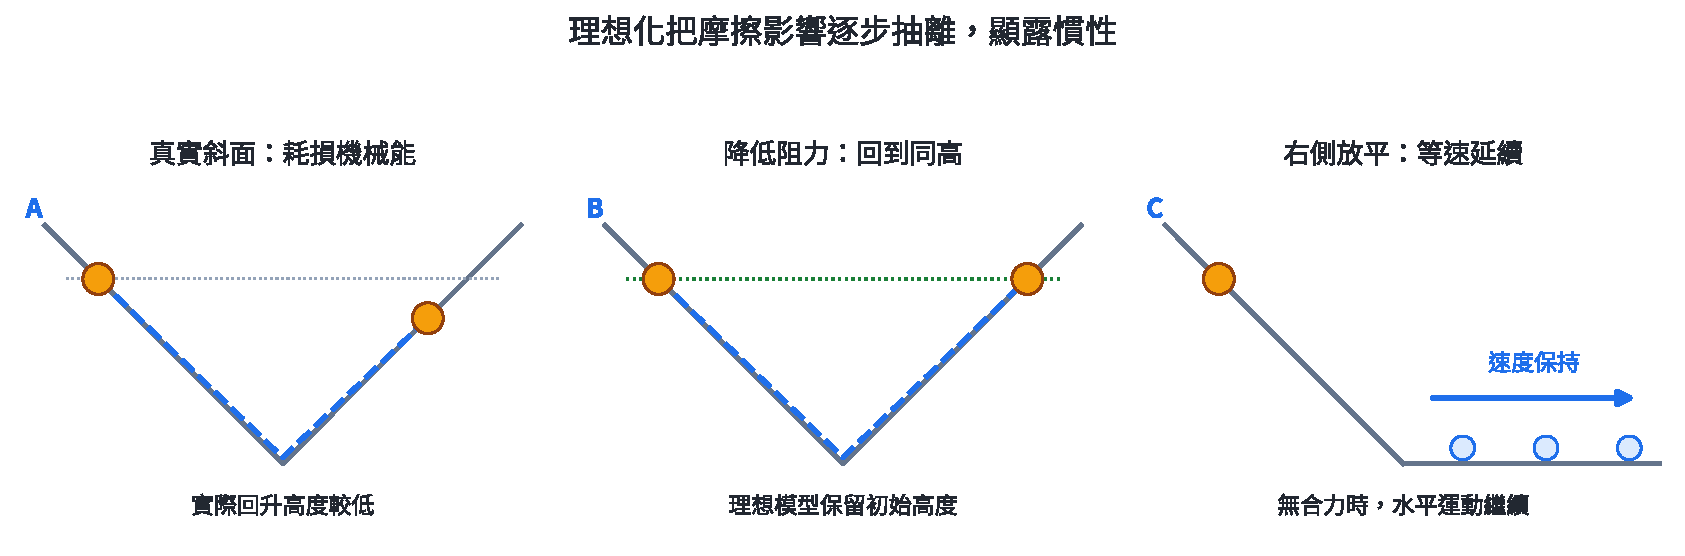
\includegraphics[width=0.98\linewidth,height=\textheight,keepaspectratio,alt={圖 1｜三個狀態逐步抽離阻力；右側放平時，球以保持速度來延續原運動狀態。}]{assets/必物-3-伽利略理想化.pdf}
\caption{圖 1｜三個狀態逐步抽離阻力；右側放平時，球以保持速度來延續原運動狀態。}
\end{figure}

這種方法的重點是控制變因與理想化：實驗告訴我們「阻力變小時，運動狀態如何變化」；理想模型再預測「阻力趨近零的極限狀態」。後面的慣性定律就是這項模型的精確表達。

\subsection{實務連結｜建模與工程判定}\label{ux5be6ux52d9ux9023ux7d50ux5efaux6a21ux8207ux5de5ux7a0bux5224ux5b9a}

車輛滑行、電梯啟動、衛星繞行都同時受很多影響。工程分析先留下會主導結果的互動，建立最小可用模型；若預測與量測差異大於容許範圍，再納入空氣阻力、滾動阻力或其他次要因素。

\clearpage

\section{2. 位置、位移、速度與加速度}\label{ux4f4dux7f6eux4f4dux79fbux901fux5ea6ux8207ux52a0ux901fux5ea6}

\subsection{2.1 參考系與一維座標}\label{ux53c3ux8003ux7cfbux8207ux4e00ux7dadux5ea7ux6a19}

「物體在移動」必須相對於某個參考系才有意義。路旁觀察者會看到乘客跟著列車向東移動；車內觀察者則可把坐在椅上的乘客視為靜止。選定參考系後，再設定原點、正方向與單位，才能用座標 \(x\) 描述位置。

{\def\LTcaptype{none} % do not increment counter
\begin{longtable}[]{@{}
  >{\raggedright\arraybackslash}p{(\linewidth - 6\tabcolsep) * \real{0.2500}}
  >{\raggedright\arraybackslash}p{(\linewidth - 6\tabcolsep) * \real{0.2500}}
  >{\raggedright\arraybackslash}p{(\linewidth - 6\tabcolsep) * \real{0.2500}}
  >{\raggedright\arraybackslash}p{(\linewidth - 6\tabcolsep) * \real{0.2500}}@{}}
\toprule\noalign{}
\begin{minipage}[b]{\linewidth}\raggedright
物理量
\end{minipage} & \begin{minipage}[b]{\linewidth}\raggedright
定義
\end{minipage} & \begin{minipage}[b]{\linewidth}\raggedright
一維表示
\end{minipage} & \begin{minipage}[b]{\linewidth}\raggedright
SI 單位
\end{minipage} \\
\midrule\noalign{}
\endhead
\bottomrule\noalign{}
\endlastfoot
位置 & 相對原點的有向座標 & \(x\) & m \\
位移 & 末位置減初位置 & \(\Delta x=x_f-x_i\) & m \\
路徑長 & 沿實際路徑累加的長度 & \(s=\sum |\Delta x_j|\) & m \\
平均速度 & 單位時間的位移 & \(\bar v=\Delta x/\Delta t\) & m/s \\
平均速率 & 單位時間的路徑長 & \(\bar u=s/\Delta t\) & m/s \\
瞬時速度 & 極短時間內的平均速度極限 & \(v\) & m/s \\
平均加速度 & 單位時間的速度變化 & \(\bar a=\Delta v/\Delta t\) & m/s\(^2\) \\
\end{longtable}
}

位移是有方向的量，一維中用正負號表示方向。路徑長與速率表示累計長度及其變化快慢，數值取非負。

\begin{figure}
\centering
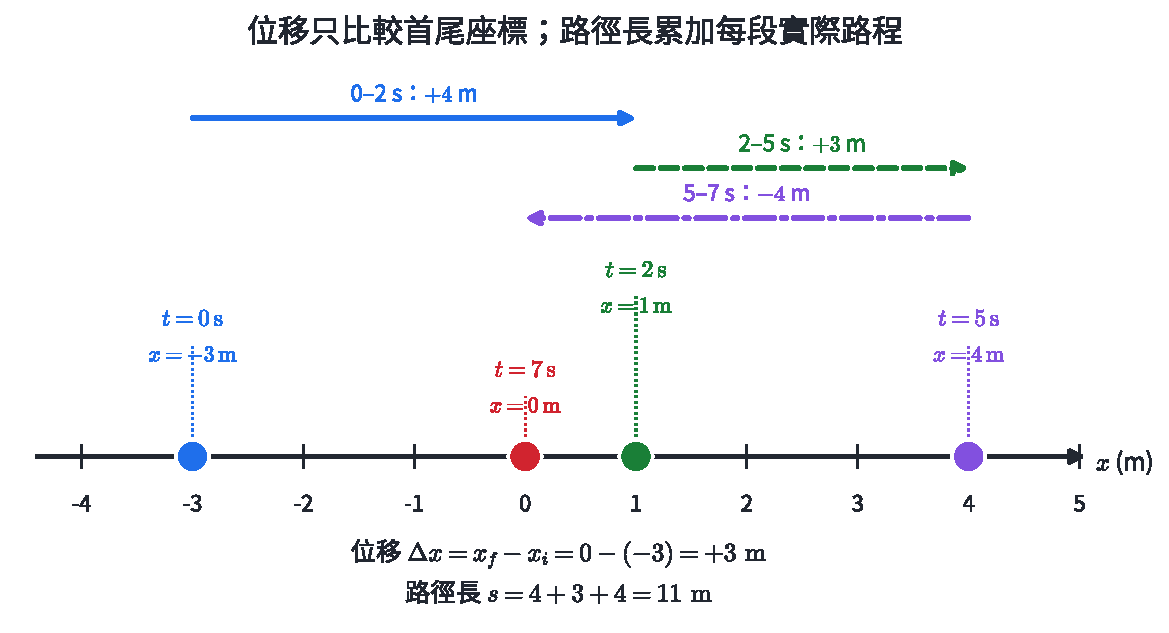
\includegraphics[width=0.96\linewidth,height=\textheight,keepaspectratio,alt={圖 2｜同一物體的四個時間狀態；三段位移分層顯示時間區間與正負方向。位移只用首尾座標，路徑長依實際往返逐段累加。}]{assets/必物-3-等時間位置與座標.pdf}
\caption{圖 2｜同一物體的四個時間狀態；三段位移分層顯示時間區間與正負方向。位移只用首尾座標，路徑長依實際往返逐段累加。}
\end{figure}

\subsection{2.2 位移與路徑長的推理}\label{ux4f4dux79fbux8207ux8defux5f91ux9577ux7684ux63a8ux7406}

把整段運動切成 \(n\) 段，第 \(j\) 段位移為 \(\Delta x_j=x_j-x_{j-1}\)。全程位移相加時，中間座標會成對抵消：

\[
\sum_{j=1}^{n}\Delta x_j
=(x_1-x_0)+(x_2-x_1)+\cdots +(x_n-x_{n-1})
=x_n-x_0.
\]

因此位移只由首尾位置決定。路徑長先對每段取絕對值再相加，方向反轉時仍會累加路程。這個差異決定平均速度可以為零，而同一趟旅程的平均速率仍為正。

\begin{HandoutWorkedExample}

\subsection{完整示範 1｜往返運動的平均速度與速率}\label{ux5b8cux6574ux793aux7bc4-1ux5f80ux8fd4ux904bux52d5ux7684ux5e73ux5747ux901fux5ea6ux8207ux901fux7387}

圖 2 中，物體在 \(t=0\) 位於 \(x=-3\ \mathrm m\)，依序移到 \(x=1\ \mathrm m\)、\(4\ \mathrm m\)，最後於 \(t=7\ \mathrm s\) 到達 \(x=0\)。

\[
\Delta x=x_f-x_i=0-(-3)=+3\ \mathrm m,
\]

\[
s=|1-(-3)|+|4-1|+|0-4|=4+3+4=11\ \mathrm m.
\]

所以

\[
\bar v=\frac{3}{7}=+0.429\ \mathrm{m/s},
\qquad
\bar u=\frac{11}{7}=1.57\ \mathrm{m/s}.
\]

正號說明首尾位移朝 \(+x\)；\(1.57\ \mathrm{m/s}\) 描述全程累計移動的快慢。

\end{HandoutWorkedExample}

\begin{HandoutWorkedExample}

\subsection{完整示範 2｜用短時間資料估計瞬時速度}\label{ux5b8cux6574ux793aux7bc4-2ux7528ux77edux6642ux9593ux8cc7ux6599ux4f30ux8a08ux77acux6642ux901fux5ea6}

一輛車在直線上的位置記錄如下：

{\def\LTcaptype{none} % do not increment counter
\begin{longtable}[]{@{}rrrrrr@{}}
\toprule\noalign{}
\(t\) (s) & 1.8 & 1.9 & 2.0 & 2.1 & 2.2 \\
\midrule\noalign{}
\endhead
\bottomrule\noalign{}
\endlastfoot
\(x\) (m) & 3.24 & 3.61 & 4.00 & 4.41 & 4.84 \\
\end{longtable}
}

以 \(t=2.0\ \mathrm s\) 左右各 \(0.1\ \mathrm s\) 的資料估計：

\[
v(2.0\ \mathrm s)\approx
\frac{x(2.1)-x(1.9)}{2.1-1.9}
=\frac{4.41-3.61}{0.20}
=4.0\ \mathrm{m/s}.
\]

若改用 \(1.8\) 至 \(2.2\ \mathrm s\)，也得 \((4.84-3.24)/0.40=4.0\ \mathrm{m/s}\)。這份資料符合 \(x=t^2\)，在 \(t=2\ \mathrm s\) 附近縮短取樣區間時，區間平均速度趨近當下速度 \(4.0\ \mathrm{m/s}\)。

\end{HandoutWorkedExample}

\subsection{2.3 加速度描述速度的變化}\label{ux52a0ux901fux5ea6ux63cfux8ff0ux901fux5ea6ux7684ux8b8aux5316}

\[
\bar a=\frac{v_f-v_i}{t_f-t_i}.
\]

加速度的正負由座標正方向決定。判斷速率變化時，同時比較 \(v\) 與 \(a\) 的方向：

\begin{itemize}
\tightlist
\item
  \(v\) 與 \(a\) 同號：速率增加。
\item
  \(v\) 與 \(a\) 異號：速率減小。
\item
  \(a=0\)：速度保持不變，可以是靜止，也可以是等速度直線運動。
\end{itemize}

\begin{HandoutWorkedExample}

\subsection{完整示範 3｜加速度方向與速率變化}\label{ux5b8cux6574ux793aux7bc4-3ux52a0ux901fux5ea6ux65b9ux5411ux8207ux901fux7387ux8b8aux5316}

取向東為正。某車的速度在 \(4.0\ \mathrm s\) 內從 \(-12\ \mathrm{m/s}\) 變為 \(-4.0\ \mathrm{m/s}\)：

\[
\bar a=\frac{-4.0-(-12)}{4.0}=+2.0\ \mathrm{m/s^2}.
\]

速度向西，加速度向東。兩者方向相反，因此速率從 \(12\) 降為 \(4.0\ \mathrm{m/s}\)。

\end{HandoutWorkedExample}

\subsection{實務連結｜GPS、區間測速與加速度感測器}\label{ux5be6ux52d9ux9023ux7d50gpsux5340ux9593ux6e2cux901fux8207ux52a0ux901fux5ea6ux611fux6e2cux5668}

GPS 依不同時刻的位置差估計速度；區間測速用兩端點距離與通過時間計算平均速率；手機內的感測器則記錄加速度隨時間的變化，用於螢幕旋轉、步態辨識與碰撞偵測。三種裝置量到的量不同，必須根據定義解讀。

\begin{HandoutSelfCheck}

\subsection{節內練習 2A｜運動量的定義}\label{ux7bc0ux5167ux7df4ux7fd2-2aux904bux52d5ux91cfux7684ux5b9aux7fa9}

\begin{enumerate}
\def\labelenumi{\arabic{enumi}.}
\tightlist
\item
  某人在 \(3.0\ \mathrm s\) 內由 \(x=-6\ \mathrm m\) 走到 \(x=9\ \mathrm m\)。求位移與平均速度。
\item
  物體由 \(x=0\) 到 \(x=4\ \mathrm m\)，再返回 \(x=3\ \mathrm m\)。求位移與路徑長。
\item
  跑者繞 \(400\ \mathrm m\) 跑道一圈回到起點，耗時 \(80\ \mathrm s\)。求平均速度與平均速率。
\item
  取向右為正，速度由 \(+6\ \mathrm{m/s}\) 在 \(2.0\ \mathrm s\) 內變為 \(-2\ \mathrm{m/s}\)。求平均加速度，並說明末狀態的運動方向。
\item
  將原點向右平移 \(100\ \mathrm m\)，同一段運動的初、末座標都減少 \(100\ \mathrm m\)。比較平移前後的位移。
\end{enumerate}

\textbf{簡答：}1. \(+15\ \mathrm m\)、\(+5.0\ \mathrm{m/s}\)。2. \(+3\ \mathrm m\)、\(5\ \mathrm m\)。3. \(0\)、\(5.0\ \mathrm{m/s}\)。4. \(-4.0\ \mathrm{m/s^2}\)，末狀態向左。5. 位移仍為 \(x_f-x_i\)，數值不變。

\end{HandoutSelfCheck}

\section{3. 運動圖與等加速度模型}\label{ux904bux52d5ux5716ux8207ux7b49ux52a0ux901fux5ea6ux6a21ux578b}

\subsection{\texorpdfstring{3.1 \(x\)--\(t\) 圖的斜率}{3.1 x--t 圖的斜率}}\label{xt-ux5716ux7684ux659cux7387}

在位置---時間圖上，兩時刻之間的割線斜率為

\[
\frac{\Delta x}{\Delta t}=\bar v.
\]

取得越接近某一時刻，割線越趨近該點的切線，切線斜率就是瞬時速度。圖線向右上升對應正速度，水平段對應靜止，向右下降對應負速度。位置在原點以下只代表 \(x<0\)，運動方向仍由斜率判定。

\subsection{\texorpdfstring{3.2 \(v\)--\(t\) 圖的斜率與面積}{3.2 v--t 圖的斜率與面積}}\label{vt-ux5716ux7684ux659cux7387ux8207ux9762ux7a4d}

在速度---時間圖上，割線斜率為 \(\Delta v/\Delta t=\bar a\)。一小段時間 \(\Delta t\) 內，若速度近似為 \(v\)，位移近似為 \(v\Delta t\)。把各小段相加，就是 \(v\)--\(t\) 圖線與時間軸間的帶號面積：

\[
\Delta x=\sum v_j\Delta t_j.
\]

時間軸上方的面積計為正，下方計為負。若要累加路徑長，則對每段面積取正值後相加。

\begin{figure}
\centering
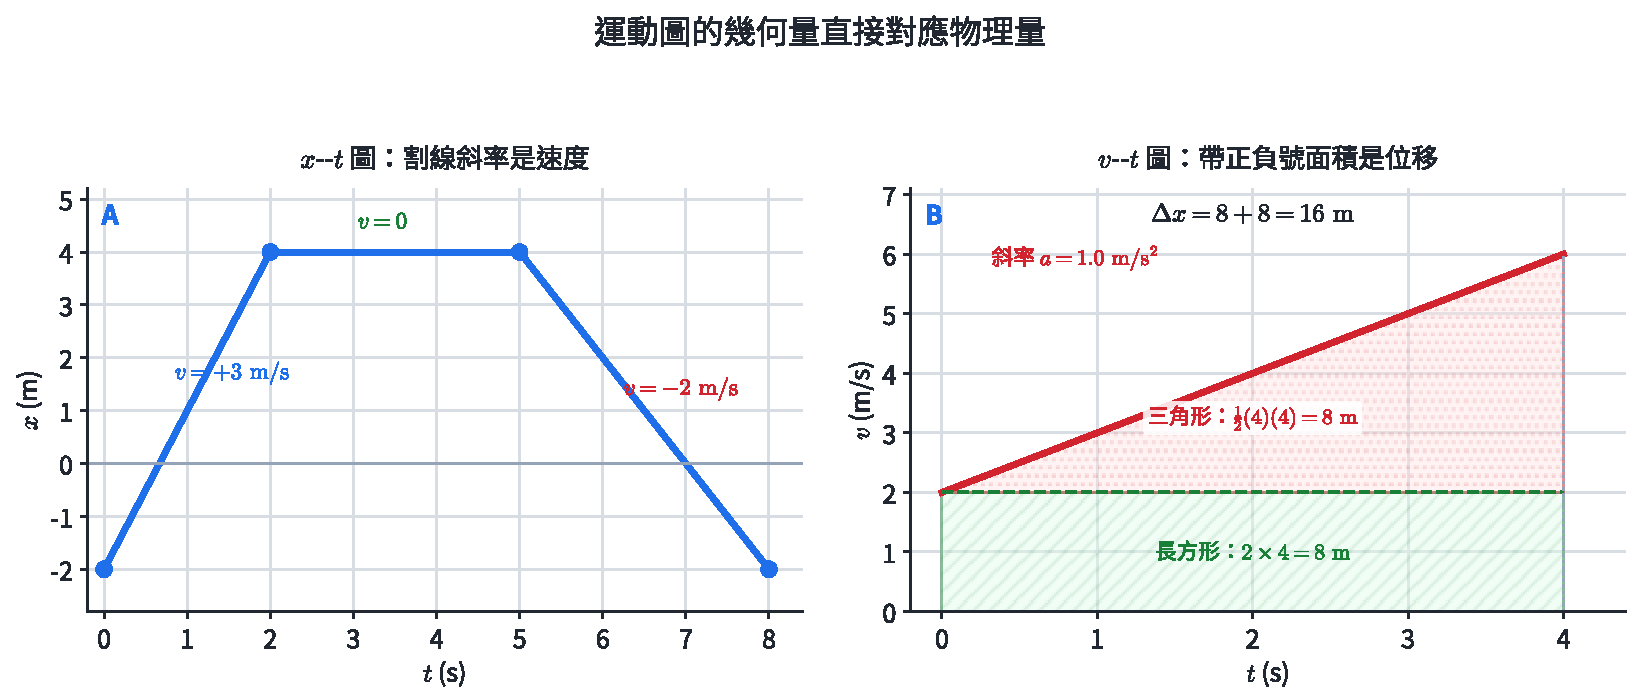
\includegraphics[width=0.98\linewidth,height=\textheight,keepaspectratio,alt={圖 3｜左圖由分段斜率讀出運動方向；右圖用不同網紋把速度圖下面積分成長方形與三角形，兩部分各代表 8\textbackslash{} \textbackslash mathrm m 位移。}]{assets/必物-3-運動圖斜率與面積.pdf}
\caption{圖 3｜左圖由分段斜率讀出運動方向；右圖用不同網紋把速度圖下面積分成長方形與三角形，兩部分各代表 \(8\ \mathrm m\) 位移。}
\end{figure}

\begin{HandoutWorkedExample}

\subsection{\texorpdfstring{完整示範 4｜讀取分段 \(x\)--\(t\) 圖}{完整示範 4｜讀取分段 x--t 圖}}\label{ux5b8cux6574ux793aux7bc4-4ux8b80ux53d6ux5206ux6bb5-xt-ux5716}

圖 3A 的位置依序為 \((0,-2)\)、\((2,4)\)、\((5,4)\)、\((8,-2)\)，座標單位分別為秒與公尺。

\[
v_1=\frac{4-(-2)}{2-0}=+3\ \mathrm{m/s},
\qquad
v_2=0,
\]

\[
v_3=\frac{-2-4}{8-5}=-2\ \mathrm{m/s}.
\]

末位置與初位置相同，所以全程位移為 \(0\)。路徑長為 \(6+0+6=12\ \mathrm m\)。

\end{HandoutWorkedExample}

\begin{HandoutWorkedExample}

\subsection{\texorpdfstring{完整示範 5｜由 \(v\)--\(t\) 圖同時求加速度與位移}{完整示範 5｜由 v--t 圖同時求加速度與位移}}\label{ux5b8cux6574ux793aux7bc4-5ux7531-vt-ux5716ux540cux6642ux6c42ux52a0ux901fux5ea6ux8207ux4f4dux79fb}

圖 3B 中，速度在 \(4.0\ \mathrm s\) 內由 \(2.0\ \mathrm{m/s}\) 線性增至 \(6.0\ \mathrm{m/s}\)。

\[
a=\frac{6.0-2.0}{4.0}=1.0\ \mathrm{m/s^2}.
\]

\[
\Delta x=(2.0)(4.0)+\frac{1}{2}(4.0)(4.0)=8.0+8.0=16\ \mathrm m.
\]

線性變化時 \(\bar v=(2.0+6.0)/2=4.0\ \mathrm{m/s}\)，因此 \(\Delta x=\bar v\Delta t=16\ \mathrm m\)，與面積法一致。

\end{HandoutWorkedExample}

\subsection{3.3 等加速度的兩個主要關係}\label{ux7b49ux52a0ux901fux5ea6ux7684ux5169ux500bux4e3bux8981ux95dcux4fc2}

等加速度指加速度在考察時間內保持不變。從 \(v\)--\(t\) 圖的固定斜率可得

\[
a=\frac{v-v_0}{t}
\quad\Rightarrow\quad
\boxed{v=v_0+at}.
\]

圖下面積為長方形 \(v_0t\) 加三角形 \(\frac{1}{2}(at)t\)，因此

\[
\boxed{\Delta x=v_0t+\frac{1}{2}at^2}.
\]

若從靜止出發，\(v_0=0\)，上式化為 \(v=at\)、\(\Delta x=\frac{1}{2}at^2\)。公式的正負號來自同一組座標約定。

\begin{HandoutWorkedExample}

\subsection{完整示範 6｜反應距離與制動距離}\label{ux5b8cux6574ux793aux7bc4-6ux53cdux61c9ux8dddux96e2ux8207ux5236ux52d5ux8dddux96e2}

車速為 \(20\ \mathrm{m/s}\)。駕駛從看到障礙到開始制動需 \(0.75\ \mathrm s\)，此期間近似保持原速。之後車輛以 \(a=-5.0\ \mathrm{m/s^2}\) 等加速度制動至停止。

\[
d_r=vt=(20)(0.75)=15\ \mathrm m.
\]

制動時間由 \(0=20-5.0t_b\) 得 \(t_b=4.0\ \mathrm s\)。制動期間的平均速度為 \((20+0)/2=10\ \mathrm{m/s}\)，所以

\[
d_b=(10)(4.0)=40\ \mathrm m.
\]

從發現障礙到停車共需 \(15+40=55\ \mathrm m\)。反應時間不變時，反應距離與車速成正比；制動距離還會受胎路摩擦、坡度與制動系統影響。

\end{HandoutWorkedExample}

\subsection{3.4 自由落體是近地面的等加速度模型}\label{ux81eaux7531ux843dux9ad4ux662fux8fd1ux5730ux9762ux7684ux7b49ux52a0ux901fux5ea6ux6a21ux578b}

忽略空氣阻力時，近地面物體只受重力，加速度向下，大小約為 \(g=9.8\ \mathrm{m/s^2}\)，估算題常取 \(g=10\ \mathrm{m/s^2}\)。圖 4 取向下為正，從靜止釋放時 \(v=gt\)、\(y=\frac{1}{2}gt^2\)。

\begin{figure}
\centering
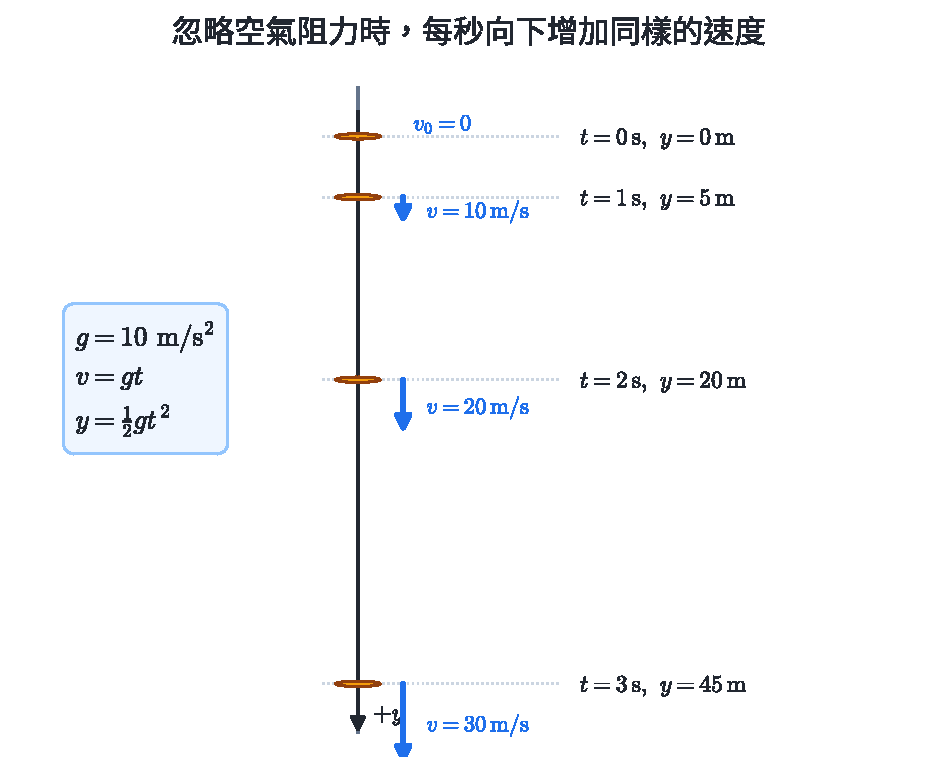
\includegraphics[width=0.8\linewidth,height=\textheight,keepaspectratio,alt={圖 4｜向下為正的自由落體。各球的位置依 t\^{}2 增加，速度箭頭依 t 增長。}]{assets/必物-3-自由落體時間狀態.pdf}
\caption{圖 4｜向下為正的自由落體。各球的位置依 \(t^2\) 增加，速度箭頭依 \(t\) 增長。}
\end{figure}

\begin{HandoutWorkedExample}

\subsection{完整示範 7｜由高度與速度交叉驗證落下時間}\label{ux5b8cux6574ux793aux7bc4-7ux7531ux9ad8ux5ea6ux8207ux901fux5ea6ux4ea4ux53c9ux9a57ux8b49ux843dux4e0bux6642ux9593}

小球從靜止釋放，忽略空氣阻力，取 \(g=10\ \mathrm{m/s^2}\)。問落下 \(20\ \mathrm m\) 所需時間與當時速度。

\[
20=\frac{1}{2}(10)t^2
\quad\Rightarrow\quad
t=2.0\ \mathrm s,
\]

\[
v=gt=(10)(2.0)=20\ \mathrm{m/s},
\]

方向向下。用平均速度驗算：\((0+20)/2=10\ \mathrm{m/s}\)，在 \(2.0\ \mathrm s\) 內位移為 \(20\ \mathrm m\)，與題意相符。

\end{HandoutWorkedExample}

\subsection{圖像讀值的必要區分}\label{ux5716ux50cfux8b80ux503cux7684ux5fc5ux8981ux5340ux5206}

\begin{itemize}
\tightlist
\item
  \(x\)--\(t\) 圖的高度是位置，斜率才是速度。
\item
  \(v\)--\(t\) 圖的高度是速度，斜率是加速度，圖下帶號面積是位移。
\end{itemize}

這個區分會直接改變答案的物理量與單位。

\begin{HandoutSelfCheck}

\subsection{節內練習 3A｜斜率、面積與等加速度}\label{ux7bc0ux5167ux7df4ux7fd2-3aux659cux7387ux9762ux7a4dux8207ux7b49ux52a0ux901fux5ea6}

\begin{enumerate}
\def\labelenumi{\arabic{enumi}.}
\tightlist
\item
  \(x\)--\(t\) 圖在 \(t=1\) 至 \(4\ \mathrm s\) 間由 \(x=2\) 線性增至 \(x=11\ \mathrm m\)。求速度。
\item
  某 \(x\)--\(t\) 圖在 \(3\ \mathrm s\) 內保持水平。這段的位移與速度各為何？
\item
  \(v\)--\(t\) 圖在 \(0\) 至 \(2\ \mathrm s\) 保持 \(+4\ \mathrm{m/s}\)，\(2\) 至 \(4\ \mathrm s\) 保持 \(-1\ \mathrm{m/s}\)。求位移與路徑長。
\item
  物體由靜止出發，以 \(a=3.0\ \mathrm{m/s^2}\) 運動 \(4.0\ \mathrm s\)。求末速度與位移。
\item
  車輛以 \(15\ \mathrm{m/s}\) 行駛，反應時間 \(0.80\ \mathrm s\)。求反應距離。
\item
  小球由靜止自由落下 \(3.0\ \mathrm s\)，取 \(g=10\ \mathrm{m/s^2}\)。求落下距離與末速率。
\end{enumerate}

\textbf{簡答：}1. \(+3.0\ \mathrm{m/s}\)。2. \(0\)、\(0\)。3. \(+6\ \mathrm m\)、\(10\ \mathrm m\)。4. \(12\ \mathrm{m/s}\)、\(24\ \mathrm m\)。5. \(12\ \mathrm m\)。6. \(45\ \mathrm m\)、\(30\ \mathrm{m/s}\) 向下。

\end{HandoutSelfCheck}

\section{4. 牛頓三大運動定律}\label{ux725bux9813ux4e09ux5927ux904bux52d5ux5b9aux5f8b}

\subsection{4.1 第一定律：合力為零時的運動狀態}\label{ux7b2cux4e00ux5b9aux5f8bux5408ux529bux70baux96f6ux6642ux7684ux904bux52d5ux72c0ux614b}

在可套用牛頓定律的參考系中，若物體所受合力為零，它會保持靜止或等速度直線運動：

\[
\sum\vec F=\vec 0
\quad\Rightarrow\quad
\vec v=\text{常向量}.
\]

物體維持原運動狀態的性質稱為\textbf{慣性}，質量是慣性大小的量度。圖 1 的理想水平軌道提供這條定律的建模脈絡：移除造成速度變化的合力後，原有速度就保留。

\subsection{4.2 第二定律：合力決定加速度}\label{ux7b2cux4e8cux5b9aux5f8bux5408ux529bux6c7aux5b9aux52a0ux901fux5ea6}

同一物體上所有外力的向量和，決定物體的加速度：

\[
\boxed{\sum\vec F=m\vec a}.
\]

圖 5A 保持質量不變，\(a\)--\(F\) 資料為通過原點的直線，顯示 \(a\propto F\)。同一合力下，\(2.0\ \mathrm{kg}\) 車的加速度是 \(1.0\ \mathrm{kg}\) 車的一半，顯示 \(a\propto1/m\)。圖 5B 反過來顯示，若要保持同一加速度，所需合力與質量成正比。

\begin{figure}
\centering
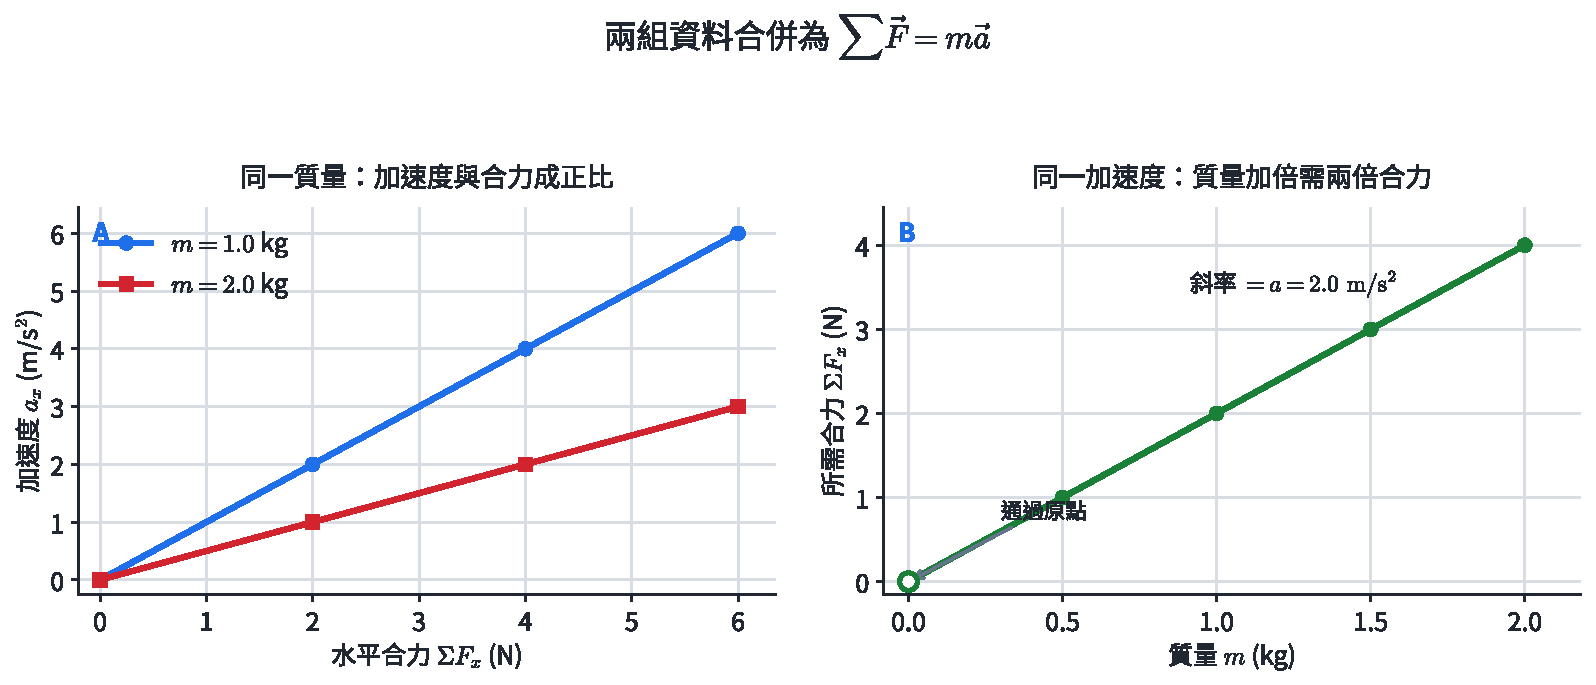
\includegraphics[width=0.96\linewidth,height=\textheight,keepaspectratio,alt={圖 5｜左圖固定質量改變合力；右圖固定加速度改變質量，並把比例線延伸到原點。兩組實驗關係共同得到 \textbackslash sum\textbackslash vec F=m\textbackslash vec a。}]{assets/必物-3-牛頓第二定律資料.pdf}
\caption{圖 5｜左圖固定質量改變合力；右圖固定加速度改變質量，並把比例線延伸到原點。兩組實驗關係共同得到 \(\sum\vec F=m\vec a\)。}
\end{figure}

牛頓（N）的定義來自第二定律：

\[
1\ \mathrm N=1\ \mathrm{kg\,m/s^2}.
\]

式中的 \(\sum\vec F\) 是合力，方向與 \(\vec a\) 相同。速度 \(\vec v\) 描述當下的運動，合力描述速度將怎麼變。

\begin{HandoutWorkedExample}

\subsection{完整示範 8｜由實驗資料求質量並預測加速度}\label{ux5b8cux6574ux793aux7bc4-8ux7531ux5be6ux9a57ux8cc7ux6599ux6c42ux8ceaux91cfux4e26ux9810ux6e2cux52a0ux901fux5ea6}

某台車在水平方向受合力 \(2.0\ \mathrm N\) 時，加速度為 \(0.80\ \mathrm{m/s^2}\)。

\[
m=\frac{F}{a}=\frac{2.0}{0.80}=2.5\ \mathrm{kg}.
\]

換成 \(5.0\ \mathrm N\) 的同方向合力後，

\[
a=\frac{5.0}{2.5}=2.0\ \mathrm{m/s^2}.
\]

單位驗算：\(\mathrm N/\mathrm{kg}=\mathrm{m/s^2}\)，符合加速度單位。

\end{HandoutWorkedExample}

\begin{HandoutWorkedExample}

\subsection{完整示範 9｜合力與速度可以方向相反}\label{ux5b8cux6574ux793aux7bc4-9ux5408ux529bux8207ux901fux5ea6ux53efux4ee5ux65b9ux5411ux76f8ux53cd}

取向右為正。質量 \(4.0\ \mathrm{kg}\) 的物體當下以 \(v=+6.0\ \mathrm{m/s}\) 運動，受到向左 \(8.0\ \mathrm N\) 的合力。

\[
a=\frac{\sum F_x}{m}=\frac{-8.0}{4.0}=-2.0\ \mathrm{m/s^2}.
\]

經 \(2.0\ \mathrm s\) 後，

\[
v=v_0+at=6.0+(-2.0)(2.0)=2.0\ \mathrm{m/s}.
\]

物體仍向右，速率已由 \(6.0\) 降為 \(2.0\ \mathrm{m/s}\)。合力向左的直接結果是加速度向左，運動方向要由後續速度判斷。

\end{HandoutWorkedExample}

\subsection{4.3 第三定律：力來自兩物體的互動}\label{ux7b2cux4e09ux5b9aux5f8bux529bux4f86ux81eaux5169ux7269ux9ad4ux7684ux4e92ux52d5}

物體 A 對物體 B 施力時，B 同時對 A 施以大小相等、方向相反、同一種互動的力：

\[
\boxed{\vec F_{A\to B}=-\vec F_{B\to A}}.
\]

這兩力同時出現，分別作用在 B 與 A 上。比較單一物體的運動時，只相加作用在該物體上的力。

\begin{figure}
\centering
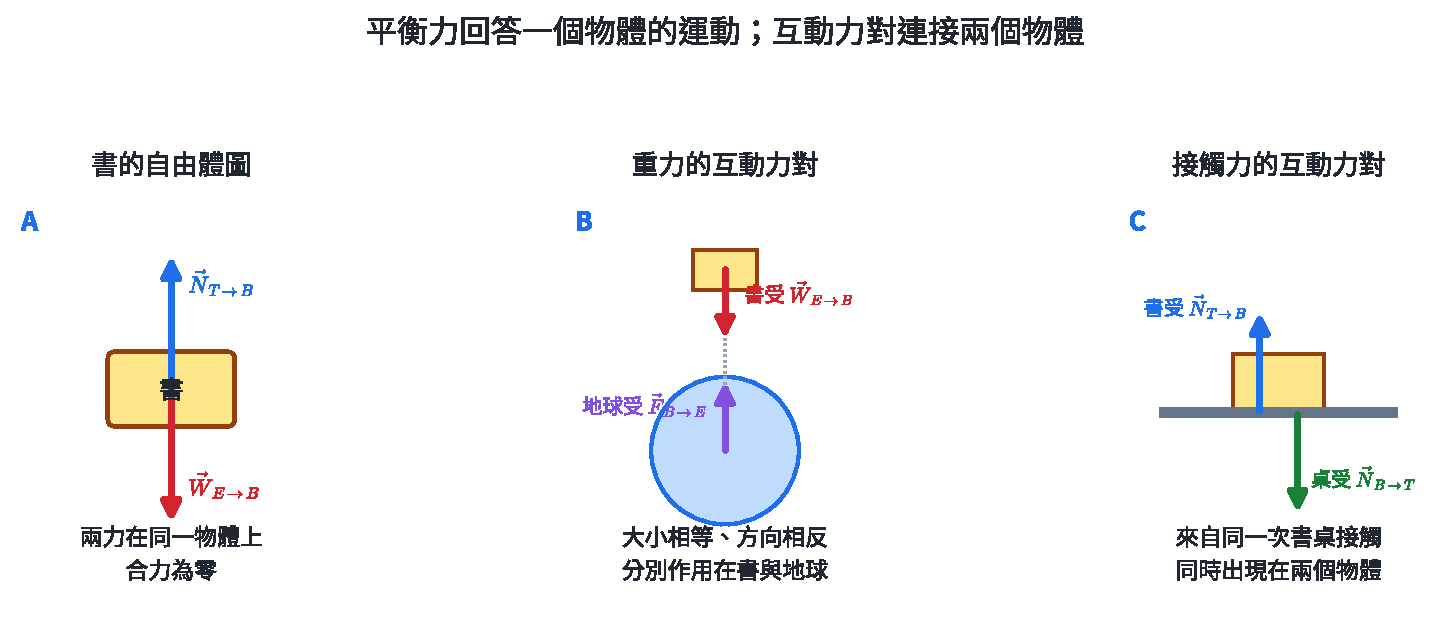
\includegraphics[width=0.98\linewidth,height=\textheight,keepaspectratio,alt={圖 6｜A 是書的受力圖；B、C 的每對箭頭分別由兩個受力物體出發，等長且反向，對應同一次重力或接觸互動。B、T、E 分別代表書、桌與地球。}]{assets/必物-3-平衡力與第三定律.pdf}
\caption{圖 6｜A 是書的受力圖；B、C 的每對箭頭分別由兩個受力物體出發，等長且反向，對應同一次重力或接觸互動。\(B\)、\(T\)、\(E\) 分別代表書、桌與地球。}
\end{figure}

圖 6A 的正向力與重力都作用在書上，在靜止條件下使書的合力為零。它們來自不同互動。各自的第三定律配對顯示在圖 6B、6C，每一對都橫跨兩個物體。

\begin{HandoutWorkedExample}

\subsection{完整示範 10｜溜冰者互推時的力相等、加速度不相等}\label{ux5b8cux6574ux793aux7bc4-10ux6e9cux51b0ux8005ux4e92ux63a8ux6642ux7684ux529bux76f8ux7b49ux52a0ux901fux5ea6ux4e0dux76f8ux7b49}

質量 \(50\ \mathrm{kg}\) 的 A 與 \(75\ \mathrm{kg}\) 的 B 在近似無摩擦的冰面互推。A 對 B 施以向右 \(150\ \mathrm N\) 的力，則 B 對 A 施以向左 \(150\ \mathrm N\) 的力。

\[
a_A=\frac{-150}{50}=-3.0\ \mathrm{m/s^2},
\qquad
a_B=\frac{+150}{75}=+2.0\ \mathrm{m/s^2}.
\]

互動力大小相等；加速度由各自質量與各自受到的合力決定，所以質量較小的 A 加速度大小較大。

\end{HandoutWorkedExample}

\subsection{實務連結｜車輛安全與機械控制}\label{ux5be6ux52d9ux9023ux7d50ux8ecaux8f1bux5b89ux5168ux8207ux6a5fux68b0ux63a7ux5236}

碰撞試驗用加速度---時間資料評估車體與乘員在短時間內的受力。在同一速度變化下，延長停止時間會降低加速度量值，這是潰縮區、安全氣囊與緩衝包裝的共同機制。機器人與自動車用加速度感測資料估計合力與路面互動，再調整驅動力。

\begin{HandoutSelfCheck}

\subsection{節內練習 4A｜牛頓三定律}\label{ux7bc0ux5167ux7df4ux7fd2-4aux725bux9813ux4e09ux5b9aux5f8b}

\begin{enumerate}
\def\labelenumi{\arabic{enumi}.}
\tightlist
\item
  太空船在遠離天體的區域燃料燃燒完畢，合力近似為零。描述後續速度。
\item
  \(3.0\ \mathrm{kg}\) 物體受向右 \(12\ \mathrm N\) 與向左 \(3.0\ \mathrm N\)。求加速度。
\item
  物體受兩個大小各 \(7.0\ \mathrm N\)、方向相反的力。求合力與加速度。
\item
  同一合力作用在 \(2.0\ \mathrm{kg}\) 與 \(6.0\ \mathrm{kg}\) 物體上。比較加速度大小。
\item
  手掌向下壓桌面 \(40\ \mathrm N\)。寫出這個力的第三定律配對。
\item
  質量 \(1000\ \mathrm{kg}\) 的車加速度為 \(1.5\ \mathrm{m/s^2}\) 向東。求水平合力。
\end{enumerate}

\textbf{簡答：}1. 大小與方向都保持。2. \(3.0\ \mathrm{m/s^2}\) 向右。3. \(0\)、\(0\)。4. \(a_{2\mathrm{kg}}:a_{6\mathrm{kg}}=3:1\)。5. 桌面同時向上推手掌 \(40\ \mathrm N\)。6. \(1.5\times10^3\ \mathrm N\) 向東。

\end{HandoutSelfCheck}

\section{5. 受力圖、平衡與常見力}\label{ux53d7ux529bux5716ux5e73ux8861ux8207ux5e38ux898bux529b}

\subsection{5.1 受力圖將互動轉成方程}\label{ux53d7ux529bux5716ux5c07ux4e92ux52d5ux8f49ux6210ux65b9ux7a0b}

受力圖（自由體圖）只保留一個受力體，再把外界對它的每一個力由物體向外畫出。建立模型的順序是：

\begin{enumerate}
\def\labelenumi{\arabic{enumi}.}
\tightlist
\item
  圈定要預測運動的物體。
\item
  列出與它互動的施力者：地球、接觸面、繩、彈簧、人或其他物體。
\item
  每一個互動畫一支力，標出符號與方向。
\item
  選擇與運動或接觸面配合的座標軸。
\item
  逐軸把圖上的力收入 \(\sum F_x=ma_x\)、\(\sum F_y=ma_y\)。
\end{enumerate}

\begin{figure}
\centering
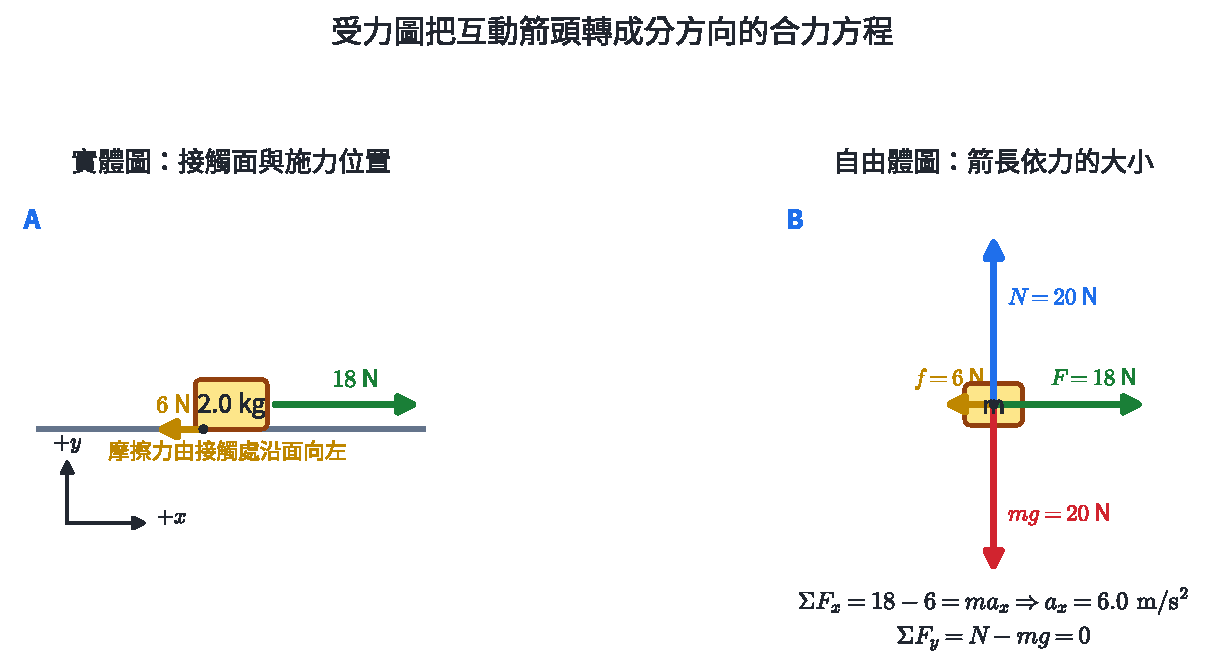
\includegraphics[width=0.98\linewidth,height=\textheight,keepaspectratio,alt={圖 7｜左圖把箱子放在接觸面上，摩擦力由接觸處沿面向左；右圖依力的大小畫箭長，水平箭長比為 18:6=3:1，鉛直兩箭頭等長。}]{assets/必物-3-水平面受力圖.pdf}
\caption{圖 7｜左圖把箱子放在接觸面上，摩擦力由接觸處沿面向左；右圖依力的大小畫箭長，水平箭長比為 \(18:6=3:1\)，鉛直兩箭頭等長。}
\end{figure}

\begin{HandoutWorkedExample}

\subsection{完整示範 11｜水平面上的合力與加速度}\label{ux5b8cux6574ux793aux7bc4-11ux6c34ux5e73ux9762ux4e0aux7684ux5408ux529bux8207ux52a0ux901fux5ea6}

圖 7 的 \(2.0\ \mathrm{kg}\) 箱子受 \(18\ \mathrm N\) 向右推力、\(6\ \mathrm N\) 向左摩擦力，取 \(g=10\ \mathrm{m/s^2}\)。水平方向：

\[
18-6=(2.0)a_x
\quad\Rightarrow\quad
a_x=6.0\ \mathrm{m/s^2}.
\]

箱子在鉛直方向無加速度：

\[
N-mg=0
\quad\Rightarrow\quad
N=(2.0)(10)=20\ \mathrm N.
\]

圖上的右向合力與計算得到的右向加速度一致；鉛直兩箭頭等長，對應鉛直合力為零。

\end{HandoutWorkedExample}

\subsection{5.2 重力與正向力}\label{ux91cdux529bux8207ux6b63ux5411ux529b}

近地面物體的重力大小為 \(W=mg\)，方向指向地心。正向力 \(N\) 是接觸面因壓縮與微觀電磁互動而對物體施加的力，方向垂直接觸面。\(N\) 的數值由鉛直運動方程決定。

\begin{figure}
\centering
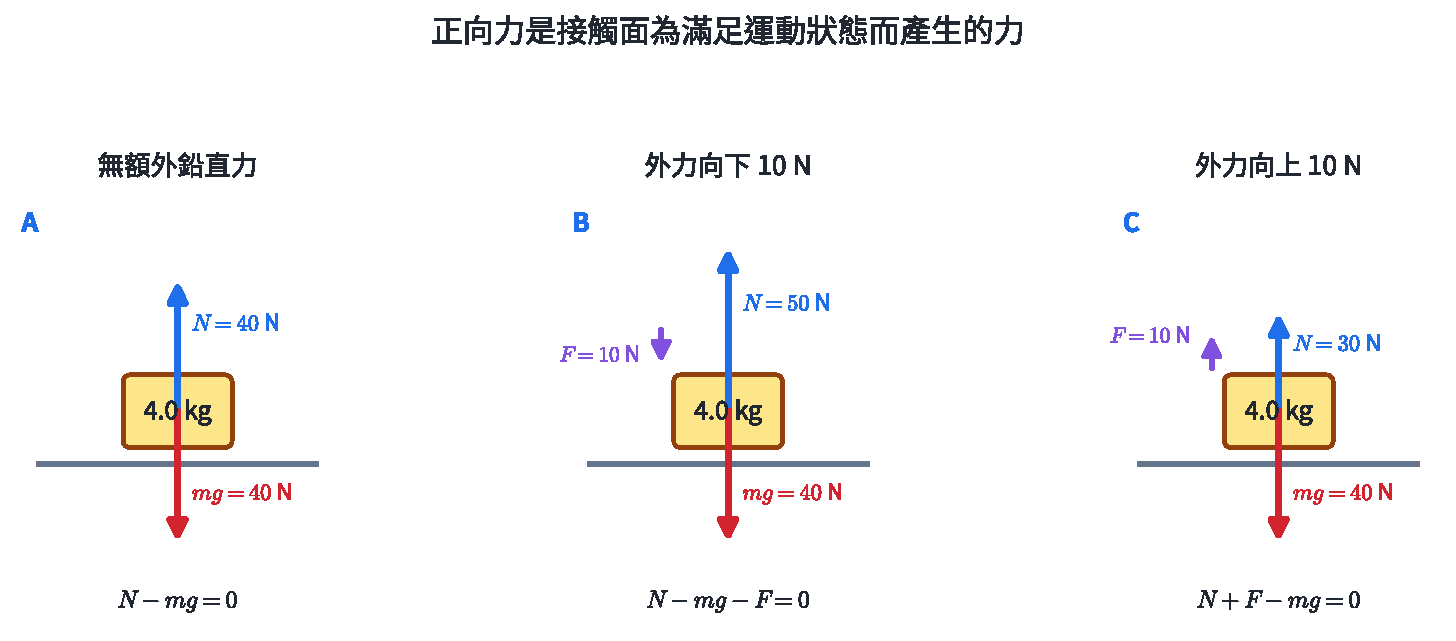
\includegraphics[width=0.98\linewidth,height=\textheight,keepaspectratio,alt={圖 8｜三個物體皆鉛直平衡。額外向下力使桌面需提供較大正向力；額外向上力分擔了一部分支撐。}]{assets/必物-3-正向力三情形.pdf}
\caption{圖 8｜三個物體皆鉛直平衡。額外向下力使桌面需提供較大正向力；額外向上力分擔了一部分支撐。}
\end{figure}

\begin{HandoutWorkedExample}

\subsection{完整示範 12｜外力改變正向力}\label{ux5b8cux6574ux793aux7bc4-12ux5916ux529bux6539ux8b8aux6b63ux5411ux529b}

質量 \(4.0\ \mathrm{kg}\) 的箱子靜止在水平桌面，取 \(g=10\ \mathrm{m/s^2}\)。

\begin{itemize}
\tightlist
\item
  只受重力與支撐時：\(N-mg=0\)，所以 \(N=40\ \mathrm N\)。
\item
  再受 \(10\ \mathrm N\) 向下外力時：\(N-mg-F=0\)，所以 \(N=50\ \mathrm N\)。
\item
  再受 \(10\ \mathrm N\) 向上外力且仍接觸桌面時：\(N+F-mg=0\)，所以 \(N=30\ \mathrm N\)。
\end{itemize}

三個結果都直接來自圖 8 的鉛直平衡方程。

\end{HandoutWorkedExample}

\subsection{5.3 彈性力與虎克定律}\label{ux5f48ux6027ux529bux8207ux864eux514bux5b9aux5f8b}

彈簧偏離自然長度時，在彈性比例限度內，彈性力大小與形變量成正比：

\[
F_s=k|\Delta L|.
\]

\(k\) 是彈簧力常數，單位為 \(\mathrm{N/m}\)。彈簧作用力方向指向恢復自然長度的方向。數據圖上 \(F\)--\(\Delta L\) 的線性區斜率就是 \(k\)。

\begin{HandoutWorkedExample}

\subsection{完整示範 13｜從伸長量求彈性力}\label{ux5b8cux6574ux793aux7bc4-13ux5f9eux4f38ux9577ux91cfux6c42ux5f48ux6027ux529b}

某彈簧在比例限度內，\(k=120\ \mathrm{N/m}\)，自然長 \(0.20\ \mathrm m\)，被拉長至 \(0.25\ \mathrm m\)。

\[
\Delta L=0.25-0.20=0.050\ \mathrm m,
\]

\[
F_s=k\Delta L=(120)(0.050)=6.0\ \mathrm N.
\]

若彈簧在物體右側被拉長，彈簧對物體的力指向右方，使彈簧長度趨向自然長。

\end{HandoutWorkedExample}

\subsection{5.4 摩擦力會配合接觸狀態}\label{ux6469ux64e6ux529bux6703ux914dux5408ux63a5ux89f8ux72c0ux614b}

摩擦力沿接觸面，方向抑制兩表面間的相對滑動或滑動趨勢。

\begin{itemize}
\tightlist
\item
  \textbf{靜摩擦力}在物體尚未滑動時自動調整，\(0\le |f_s|\le f_{s,\max}\)。
\item
  \textbf{動摩擦力}在表面相對滑動時作用；固定表面與正向力下，其大小可用近似定值描述。
\end{itemize}

\begin{figure}
\centering
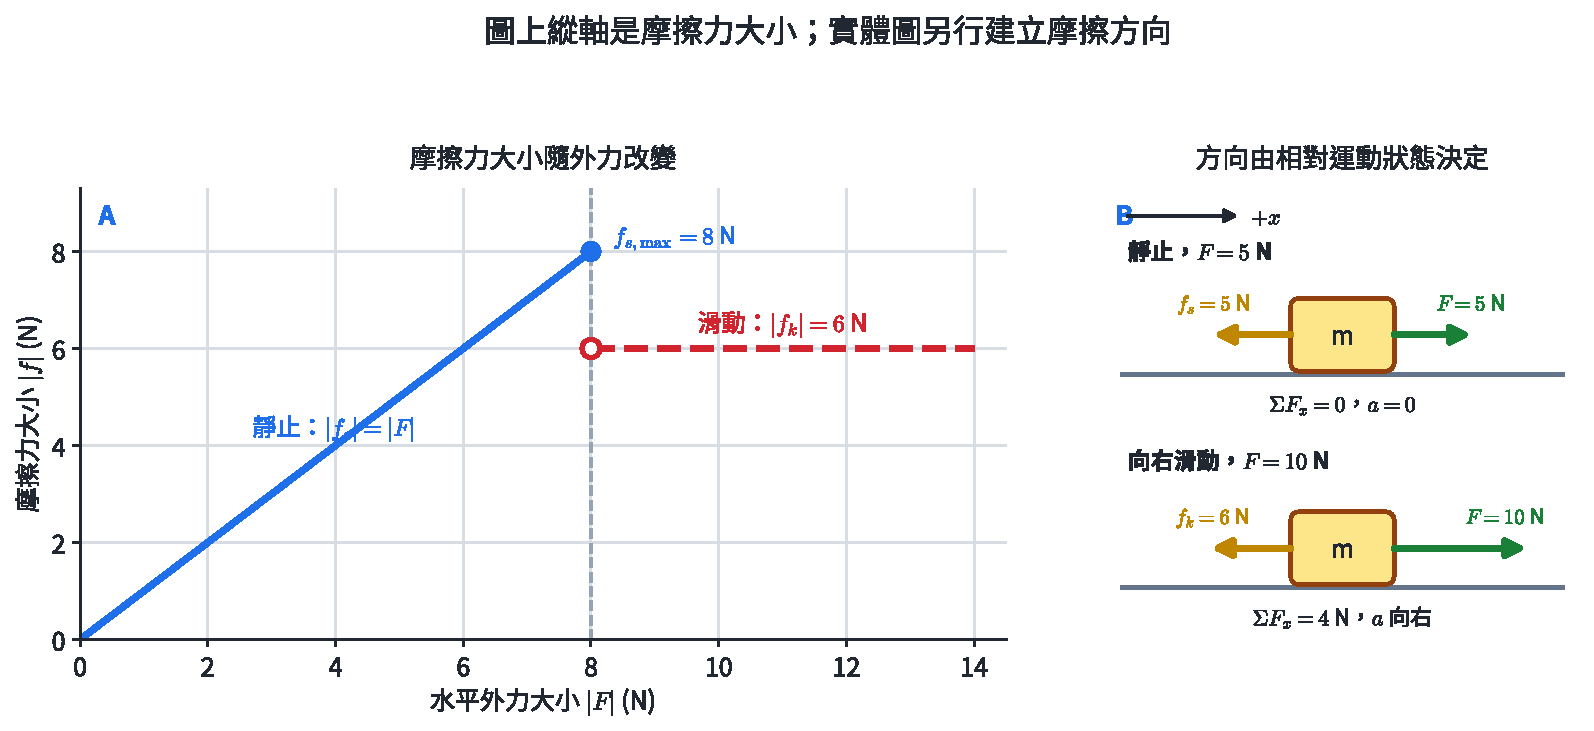
\includegraphics[width=0.94\linewidth,height=\textheight,keepaspectratio,alt={圖 9｜左圖只表示摩擦力大小，未使用面積編碼；右圖另畫方向。靜止時 f\_s 與外力等大反向，開始向右滑動後改用向左的動摩擦力。}]{assets/必物-3-摩擦力隨外力.pdf}
\caption{圖 9｜左圖只表示摩擦力大小，未使用面積編碼；右圖另畫方向。靜止時 \(f_s\) 與外力等大反向，開始向右滑動後改用向左的動摩擦力。}
\end{figure}

\begin{HandoutWorkedExample}

\subsection{完整示範 14｜先判斷靜止或滑動，再列合力}\label{ux5b8cux6574ux793aux7bc4-14ux5148ux5224ux65b7ux975cux6b62ux6216ux6ed1ux52d5ux518dux5217ux5408ux529b}

質量 \(2.0\ \mathrm{kg}\) 的物體原本靜止，圖 9 給出 \(f_{s,\max}=8\ \mathrm N\)、\(f_k=6\ \mathrm N\)。

外力為 \(5\ \mathrm N\) 時，靜摩擦力可調整為 \(5\ \mathrm N\) 且方向相反，合力為零，物體保持靜止。

外力增至 \(10\ \mathrm N\) 時，超過 \(f_{s,\max}\)，物體開始滑動，摩擦力大小為 \(6\ \mathrm N\)：

\[
\sum F_x=10-6=4\ \mathrm N,
\qquad
a=\frac{4}{2.0}=2.0\ \mathrm{m/s^2}.
\]

摩擦力的數值由接觸狀態與其容許範圍決定，再與其他力合成。

\end{HandoutWorkedExample}

\subsection{實務連結｜秤重、輪胎抓地與彈簧感測}\label{ux5be6ux52d9ux9023ux7d50ux79e4ux91cdux8f2aux80ceux6293ux5730ux8207ux5f48ux7c27ux611fux6e2c}

體重計量到的是秤與人之間的正向互動，在鉛直加速時讀數會隨 \(N-mg=ma_y\) 改變。輪胎加速、制動與轉彎所需的水平力來自路面摩擦。機械式秤與部分力感測器先校準 \(F\)--\(\Delta L\) 斜率，再用形變量反推受力。

\begin{HandoutSelfCheck}

\subsection{節內練習 5A｜常見力與受力圖}\label{ux7bc0ux5167ux7df4ux7fd2-5aux5e38ux898bux529bux8207ux53d7ux529bux5716}

\begin{enumerate}
\def\labelenumi{\arabic{enumi}.}
\tightlist
\item
  蘋果離手後在空中落下，忽略空氣阻力。列出蘋果的受力。
\item
  \(5.0\ \mathrm{kg}\) 箱子靜止在水平面，又受 \(15\ \mathrm N\) 向下外力。取 \(g=10\ \mathrm{m/s^2}\)，求 \(N\)。
\item
  \(3.0\ \mathrm{kg}\) 物體在水平面受 \(20\ \mathrm N\) 向右與 \(5\ \mathrm N\) 向左摩擦力。求加速度。
\item
  \(k=200\ \mathrm{N/m}\) 的彈簧伸長 \(3.0\ \mathrm{cm}\)。求彈性力大小。
\item
  物體原本靜止，\(f_{s,\max}=9\ \mathrm N\)。施以 \(7\ \mathrm N\) 水平外力時，求靜摩擦力大小與物體加速度。
\item
  書靜止在桌上。分別寫出「地球對書的重力」與「桌對書的正向力」的第三定律配對。
\end{enumerate}

\textbf{簡答：}1. 地球對蘋果的重力，向下。2. \(65\ \mathrm N\)。3. \(5.0\ \mathrm{m/s^2}\) 向右。4. \(6.0\ \mathrm N\)。5. \(7\ \mathrm N\) 反向、\(a=0\)。6. 書對地球的引力；書對桌面的接觸力。

\end{HandoutSelfCheck}

\section{6. 圓周運動與天體運動}\label{ux5713ux5468ux904bux52d5ux8207ux5929ux9ad4ux904bux52d5}

\subsection{6.1 等速率圓周運動仍有加速度}\label{ux7b49ux901fux7387ux5713ux5468ux904bux52d5ux4ecdux6709ux52a0ux901fux5ea6}

速度是向量。物體沿圓周以固定速率運動時，速度的大小不變，方向卻持續轉動。圖 10A 中速度沿軌道切線，加速度指向圓心。圖 10B 把相鄰時刻的兩個速度向量放在同一起點，\(\Delta\vec v\) 指向軌道內側；當時間間隔縮短，這個方向趨近圓心。

\begin{figure}
\centering
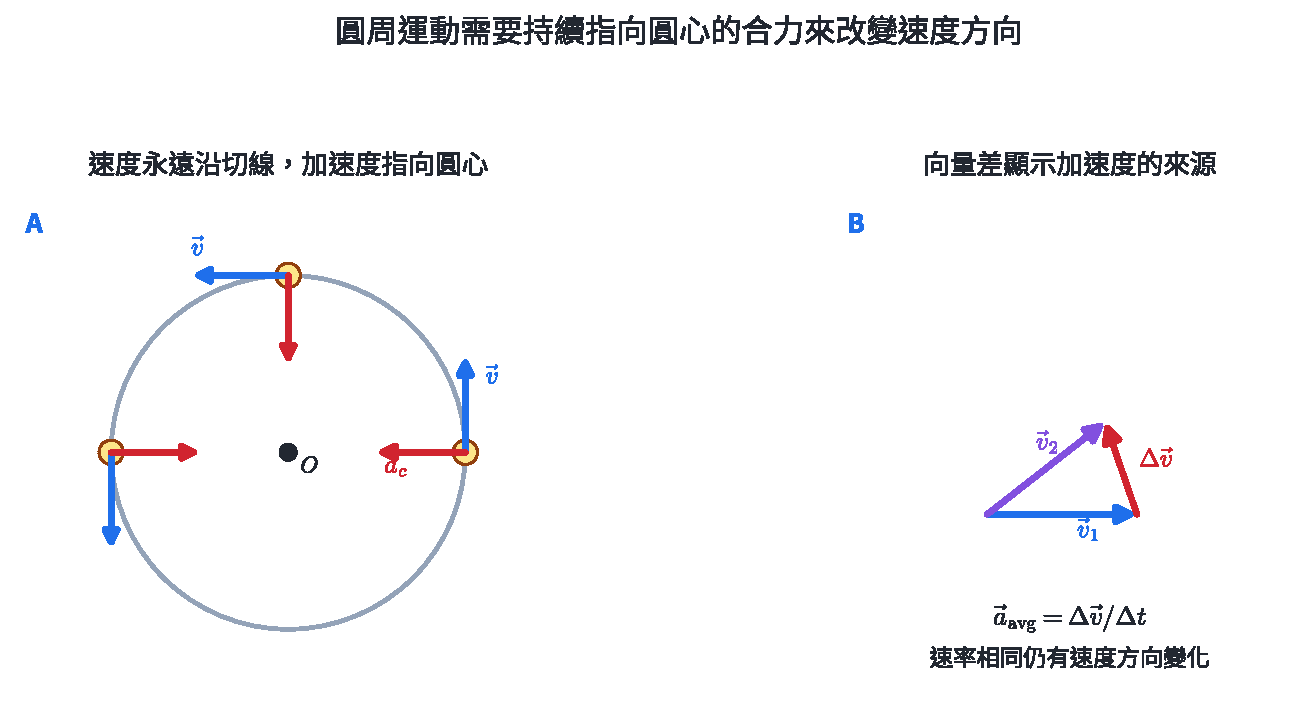
\includegraphics[width=0.94\linewidth,height=\textheight,keepaspectratio,alt={圖 10｜左圖的藍色速度箭頭等長且沿切線，紅色加速度指向圓心；右圖用速度向量差解釋加速度。}]{assets/必物-3-圓周速度與向心.pdf}
\caption{圖 10｜左圖的藍色速度箭頭等長且沿切線，紅色加速度指向圓心；右圖用速度向量差解釋加速度。}
\end{figure}

根據第二定律，加速度指向圓心表示合力也指向圓心。繩子的張力、路面摩擦、重力或正向力都可以在不同情境擔任這個徑向合力。必修範圍先掌握向量方向與合力角色；向心加速度的定量式在選修物理 I 展開。

\begin{HandoutWorkedExample}

\subsection{完整示範 15｜圈道上速度與合力的方向}\label{ux5b8cux6574ux793aux7bc4-15ux5708ux9053ux4e0aux901fux5ea6ux8207ux5408ux529bux7684ux65b9ux5411}

小車在水平圓形軌道上逆時針等速率運動。當小車位於圓的最右端時：速度沿軌道切線向上，加速度指向圓心而向左，水平合力與加速度同向。

接著到達圓的最上端時，速度轉為向左，加速度與合力轉為向下。這些方向是由軌道幾何決定的。

\end{HandoutWorkedExample}

\subsection{6.2 克卜勒三定律}\label{ux514bux535cux52d2ux4e09ux5b9aux5f8b}

克卜勒從長期行星位置資料整理出三條關係：

\begin{enumerate}
\def\labelenumi{\arabic{enumi}.}
\tightlist
\item
  \textbf{軌道定律}：行星繞太陽的軌道為橢圓，太陽在橢圓的一個焦點上。
\item
  \textbf{面積定律}：太陽與行星的連線在相等時間內掃過相等面積。行星靠近太陽時，同時間掃過的弧長較大，所以速率較大。
\item
  \textbf{週期定律}：繞同一中心天體的物體，軌道半長軸 \(a\) 的立方與週期 \(T\) 的平方成固定比：
\end{enumerate}

\[
\boxed{\frac{a^3}{T^2}=\text{常數}}
\qquad\text{或寫成}\qquad
\boxed{T^2\propto a^3}.
\]

軌道近似圓形時，\(a\) 就是軌道半徑 \(R\)。不同中心天體的質量不同，比例常數也不同，因此週期比較要先確認是繞同一中心天體。

\begin{figure}
\centering
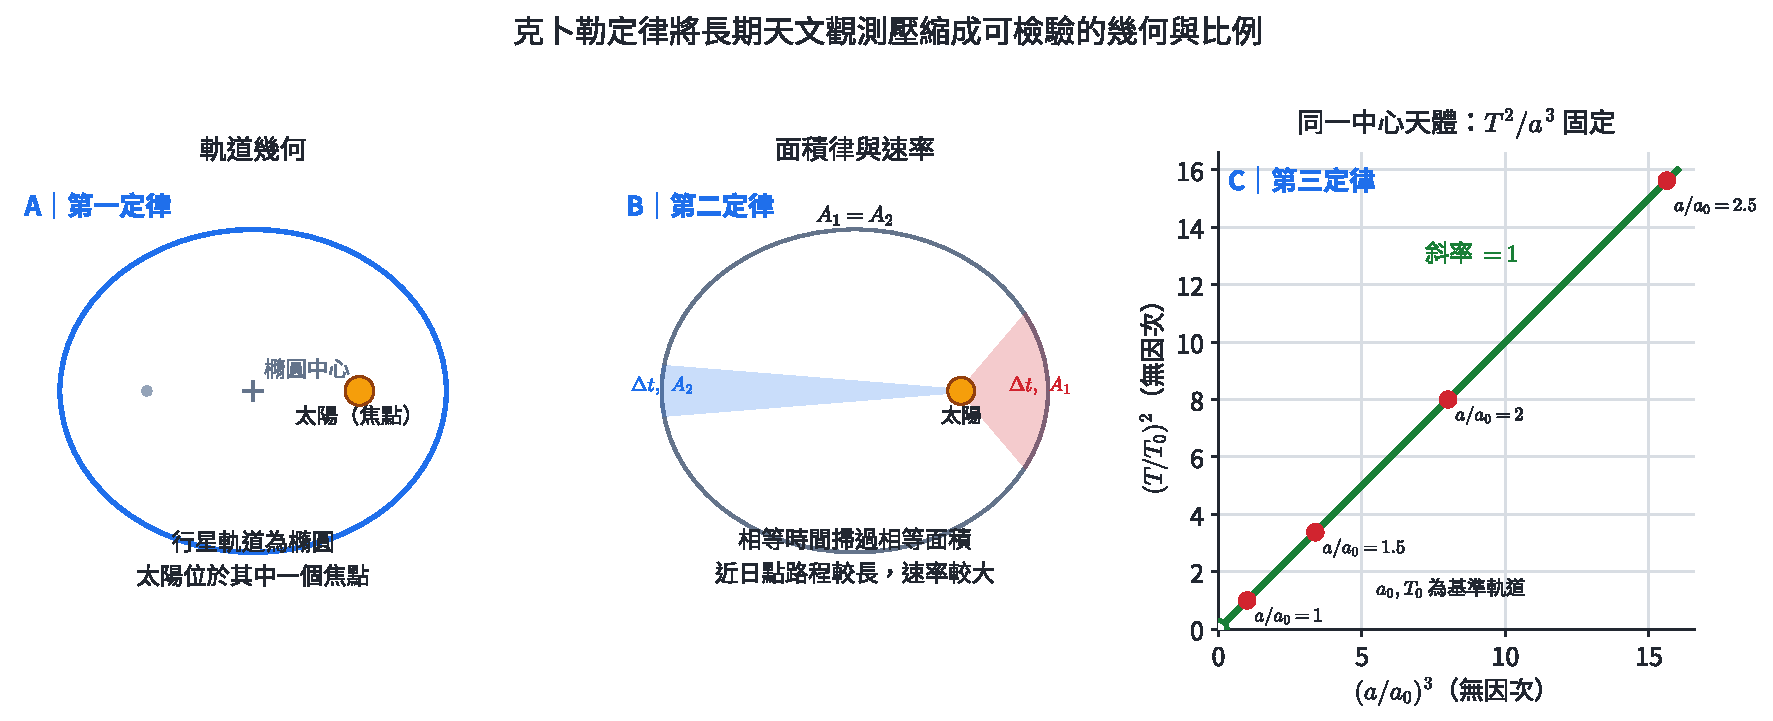
\includegraphics[width=0.98\linewidth,height=\textheight,keepaspectratio,alt={圖 11｜A 顯示太陽位於焦點；B 用不同網紋標出經數值校驗的相等時間、相等面積；C 以同一中心天體的基準軌道 (a\_0,T\_0) 正規化，直線通過原點且斜率為 1。}]{assets/必物-3-克卜勒三定律.pdf}
\caption{圖 11｜A 顯示太陽位於焦點；B 用不同網紋標出經數值校驗的相等時間、相等面積；C 以同一中心天體的基準軌道 \((a_0,T_0)\) 正規化，直線通過原點且斜率為 1。}
\end{figure}

\subsection{6.3 從觀測歸納，再用理論演繹}\label{ux5f9eux89c0ux6e2cux6b78ux7d0dux518dux7528ux7406ux8ad6ux6f14ux7e79}

克卜勒的三條定律是從大量行星觀測資料中找出共同關係，屬於\textbf{歸納}。牛頓後來用運動定律與萬有引力建立更底層的模型，再由模型推出行星軌道應符合的關係，屬於\textbf{演繹}。科學實務會在兩者間循環：觀測整理出規律，理論產生新預測，新觀測再檢驗預測。

\begin{HandoutWorkedExample}

\subsection{完整示範 16｜面積定律與軌道速率}\label{ux5b8cux6574ux793aux7bc4-16ux9762ux7a4dux5b9aux5f8bux8207ux8eccux9053ux901fux7387}

行星在軌道上由 A 移至 B 耗時 \(30\) 天，太陽連線掃過面積 \(S\)。另一段 C 至 D 也耗時 \(30\) 天。根據面積定律，C--D 掃過面積也是 \(S\)。

若 A--B 較靠近太陽，掃過區域的高（行星到太陽的距離）較短。要在同時間維持相同面積，軌道底邊對應的弧長較長，因此近日點附近的平均速率較大。

\end{HandoutWorkedExample}

\begin{HandoutWorkedExample}

\subsection{完整示範 17｜用週期定律比較兩軌道}\label{ux5b8cux6574ux793aux7bc4-17ux7528ux9031ux671fux5b9aux5f8bux6bd4ux8f03ux5169ux8eccux9053}

兩顆行星繞同一恒星運行，B 的軌道半長軸是 A 的 \(4\) 倍。

\[
\frac{a_A^3}{T_A^2}=\frac{a_B^3}{T_B^2},
\]

\[
\left(\frac{T_B}{T_A}\right)^2
=\left(\frac{a_B}{a_A}\right)^3
=4^3=64,
\]

\[
\frac{T_B}{T_A}=8.
\]

B 離中心天體較遠，週期為 A 的 \(8\) 倍。把結果代回 \(a^3/T^2\)：\(4^3/8^2=1\)，與 A 的比值相同。

\end{HandoutWorkedExample}

\subsection{實務連結｜衛星軌道與系外行星}\label{ux5be6ux52d9ux9023ux7d50ux885bux661fux8eccux9053ux8207ux7cfbux5916ux884cux661f}

衛星任務用軌道週期安排通訊窗口、地面覆蓋與觀測重訪時間。天文學家從恒星亮度週期性降低或光譜往復偏移得到系外行星週期，再結合恒星資料估計軌道尺度。克卜勒定律因此是從觀測時間序列連到天體系統結構的關鍵模型。

\begin{HandoutSelfCheck}

\subsection{節內練習 6A｜圓周方向與克卜勒定律}\label{ux7bc0ux5167ux7df4ux7fd2-6aux5713ux5468ux65b9ux5411ux8207ux514bux535cux52d2ux5b9aux5f8b}

\begin{enumerate}
\def\labelenumi{\arabic{enumi}.}
\tightlist
\item
  物體逆時針繞圓，位於圓的最上端。指出速度、加速度與合力方向。
\item
  行星位於橢圓軌道近日點與遠日點時，何處速率較大？使用面積定律說明。
\item
  兩衛星繞同一行星作近似圓軌道運動，\(R_B=9R_A\)。求 \(T_B/T_A\)。
\item
  某行星軌道半長軸是地球的 \(2\) 倍，且繞太陽運行。以地球年為單位估計週期。
\item
  先由多顆行星資料找出 \(T^2\propto a^3\)，再用此關係預測新發現行星的週期。指出前後兩個步驟分別屬於歸納或演繹。
\end{enumerate}

\textbf{簡答：}1. 速度向左，加速度與合力向下。2. 近日點；同時間等面積使近日點弧長較大。3. \(27\)。4. \(2^{3/2}\approx2.83\) 年。5. 前者歸納，後者演繹。

\end{HandoutSelfCheck}

\section{7. 核心整理}\label{ux6838ux5fc3ux6574ux7406}

\subsection{運動描述}\label{ux904bux52d5ux63cfux8ff0}

\[
\Delta x=x_f-x_i,
\qquad
\bar v=\frac{\Delta x}{\Delta t},
\qquad
\bar a=\frac{\Delta v}{\Delta t}.
\]

\begin{itemize}
\tightlist
\item
  \(x\)--\(t\) 圖斜率是速度。
\item
  \(v\)--\(t\) 圖斜率是加速度，帶號面積是位移。
\item
  等加速度：\(v=v_0+at\)、\(\Delta x=v_0t+\frac{1}{2}at^2\)。
\item
  從靜止自由落下：\(v=gt\)、\(y=\frac{1}{2}gt^2\)。
\end{itemize}

\subsection{力與運動}\label{ux529bux8207ux904bux52d5}

\[
\sum\vec F=\vec0\Rightarrow\vec v\text{ 為常向量},
\qquad
\sum\vec F=m\vec a,
\qquad
\vec F_{A\to B}=-\vec F_{B\to A}.
\]

\begin{itemize}
\tightlist
\item
  受力圖先限定一個物體，再畫外界對它的作用。
\item
  重力 \(W=mg\)；正向力垂直接觸面且由運動方程決定。
\item
  比例限度內 \(F_s=k|\Delta L|\)，方向指向恢復自然長度。
\item
  靜摩擦在 \(0\) 至 \(f_{s,\max}\) 間配合外力；滑動後使用動摩擦狀態。
\end{itemize}

\subsection{圓周與天體}\label{ux5713ux5468ux8207ux5929ux9ad4}

\begin{itemize}
\tightlist
\item
  圓周運動的速度沿切線，加速度與合力指向圓心。
\item
  克卜勒第一定律：橢圓軌道與焦點。
\item
  第二定律：等時間掃過等面積。
\item
  第三定律：繞同一中心天體時 \(a^3/T^2\) 固定。
\end{itemize}

\section{8. 代表題：分層練習}\label{ux4ee3ux8868ux984cux5206ux5c64ux7df4ux7fd2}

\subsection{A 層｜定義與單一關係}\label{a-ux5c64ux5b9aux7fa9ux8207ux55aeux4e00ux95dcux4fc2}

\textbf{題目 1｜位移、路徑長與平均量}

跑者在 \(t=0\) 位於 \(x=-20\ \mathrm m\)，\(8.0\ \mathrm s\) 後到 \(x=12\ \mathrm m\)，再於 \(t=12.0\ \mathrm s\) 到 \(x=-4\ \mathrm m\)。求全程位移、路徑長、平均速度與平均速率。

\textbf{題目 2｜速度符號與加速度}

取向右為正，某物體在 \(2.0\ \mathrm s\) 內由 \(v_i=-4.0\ \mathrm{m/s}\) 均勻變為 \(v_f=+2.0\ \mathrm{m/s}\)。求加速度，並判斷速率在整段時間內如何變化。

\textbf{題目 3｜分段 \(x\)--\(t\) 圖}

使用圖 3A，求三段速度、全程位移、路徑長與 \(0\) 至 \(8\ \mathrm s\) 的平均速度。

\textbf{題目 4｜線性 \(v\)--\(t\) 圖}

使用圖 3B，求 \(0\) 至 \(4\ \mathrm s\) 的加速度、位移與平均速度。

\textbf{題目 5｜自由落體}

一小球由靜止釋放，忽略空氣阻力，取 \(g=10\ \mathrm{m/s^2}\)。求落下 \(20\ \mathrm m\) 所需時間與當時速度。

\textbf{題目 6｜慣性}

台車上有一個水平台面，球原本與車一起靜止。若台車突然向右加速，球與台面間摩擦很小，從地面參考系與車上觀察各描述球的初期運動。

\subsection{B 層｜受力圖與定量預測}\label{b-ux5c64ux53d7ux529bux5716ux8207ux5b9aux91cfux9810ux6e2c}

\textbf{題目 7｜第二定律資料}

某車受水平合力 \(4.0\ \mathrm N\) 時，加速度為 \(2.0\ \mathrm{m/s^2}\)。求車的質量；若合力增為 \(6.0\ \mathrm N\)，求新加速度。

\textbf{題目 8｜第三定律與不同質量}

\(50\ \mathrm{kg}\) 的 A 與 \(75\ \mathrm{kg}\) 的 B 在水平冰面互推。A 對 B 施以 \(180\ \mathrm N\) 向右的力，忽略其他水平力。求 B 對 A 的力，以及 A、B 各自加速度。

\textbf{題目 9｜水平面受力圖}

\(3.0\ \mathrm{kg}\) 箱子在水平面受 \(20\ \mathrm N\) 向右推力與 \(5.0\ \mathrm N\) 向左摩擦力。取 \(g=10\ \mathrm{m/s^2}\)。畫受力圖，求正向力與水平加速度。

\textbf{題目 10｜額外鉛直外力}

\(5.0\ \mathrm{kg}\) 箱子靜止在水平地面，又受手掌 \(15\ \mathrm N\) 向下的力。取 \(g=10\ \mathrm{m/s^2}\)，求地面對箱子的正向力。

\textbf{題目 11｜彈簧校準}

彈簧力常數為 \(150\ \mathrm{N/m}\)，在比例限度內由自然長伸長 \(4.0\ \mathrm{cm}\)。求彈性力大小，並說明彈簧對右端物體的作用方向。

\textbf{題目 12｜靜摩擦與動摩擦}

\(2.0\ \mathrm{kg}\) 物體原本靜止，\(f_{s,\max}=8.0\ \mathrm N\)、\(f_k=6.0\ \mathrm N\)。分別在水平外力為 \(7.0\ \mathrm N\) 與 \(10\ \mathrm N\) 時，求摩擦力、合力與加速度。

\subsection{C 層｜向量、軌道與資料}\label{c-ux5c64ux5411ux91cfux8eccux9053ux8207ux8cc7ux6599}

\textbf{題目 13｜圓周運動的方向}

物體以固定速率逆時針繞圓。分別寫出物體在最右端與最上端時的速度、加速度與合力方向。

\textbf{題目 14｜克卜勒面積定律}

行星由近日點附近的 A 移至 B 耗時 \(20\) 天，掃過面積 \(S\)。在遠日點附近由 C 移至 D 也耗時 \(20\) 天。求 C--D 掃過面積，並比較 A--B 與 C--D 的弧長及平均速率。

\textbf{題目 15｜克卜勒週期定律}

行星 A、B 繞同一恒星運行，\(a_B=4a_A\)。求 \(T_B/T_A\)。

\textbf{題目 16｜軌道資料與科學推理}

以適當單位表示同一行星系的三顆衛星：

{\def\LTcaptype{none} % do not increment counter
\begin{longtable}[]{@{}lrr@{}}
\toprule\noalign{}
衛星 & \(a\) & \(T\) \\
\midrule\noalign{}
\endhead
\bottomrule\noalign{}
\endlastfoot
P & 1 & 1 \\
Q & 4 & 8 \\
R & 9 & 27 \\
\end{longtable}
}

計算三者 \(a^3/T^2\)，判斷資料是否支持克卜勒第三定律。從這組數據找出共同關係屬於歸納或演繹？

\subsection{跨節整合題}\label{ux8de8ux7bc0ux6574ux5408ux984c}

\textbf{整合題 1｜反應、制動與運動圖}

車輛以 \(20\ \mathrm{m/s}\) 行駛，駕駛的反應時間為 \(0.75\ \mathrm s\)，反應期間車速近似不變。制動後加速度固定為 \(-5.0\ \mathrm{m/s^2}\)，直到停止。畫 \(v\)--\(t\) 圖，求反應距離、制動時間、制動距離與總停車距離。

\textbf{整合題 2｜電梯秤讀數、受力圖與速度}

\(60\ \mathrm{kg}\) 的人站在電梯秤上，秤對人的正向力為 \(720\ \mathrm N\)，取 \(g=10\ \mathrm{m/s^2}\) 與向上為正。畫人的受力圖並求加速度。若當下電梯速度為 \(-3.0\ \mathrm{m/s}\)，加速度在接下來 \(1.0\ \mathrm s\) 保持不變，求末速度並描述速率變化。

\textbf{整合題 3｜摩擦狀態與分段運動}

\(2.0\ \mathrm{kg}\) 物體原本靜止在水平面，\(f_{s,\max}=8.0\ \mathrm N\)、\(f_k=6.0\ \mathrm N\)。先施以 \(5.0\ \mathrm N\) 向右外力 \(2.0\ \mathrm s\)，接著將外力改為 \(10\ \mathrm N\) 並維持 \(3.0\ \mathrm s\)。求兩階段的摩擦力、加速度，以及全程末速度與位移。

\textbf{整合題 4｜系外行星的週期預測}

兩顆行星 A、B 繞同一恒星作近似圓軌道運動，\(R_B=2R_A\)，A 的週期為 \(3.00\) 年。求 B 的週期。若觀測得 B 的週期為 \(8.5\) 年，比較觀測與模型預測，並說明這份結果支持的關係。

\clearpage

\section{9. 完整解析}\label{ux5b8cux6574ux89e3ux6790}

\begin{figure}
\centering
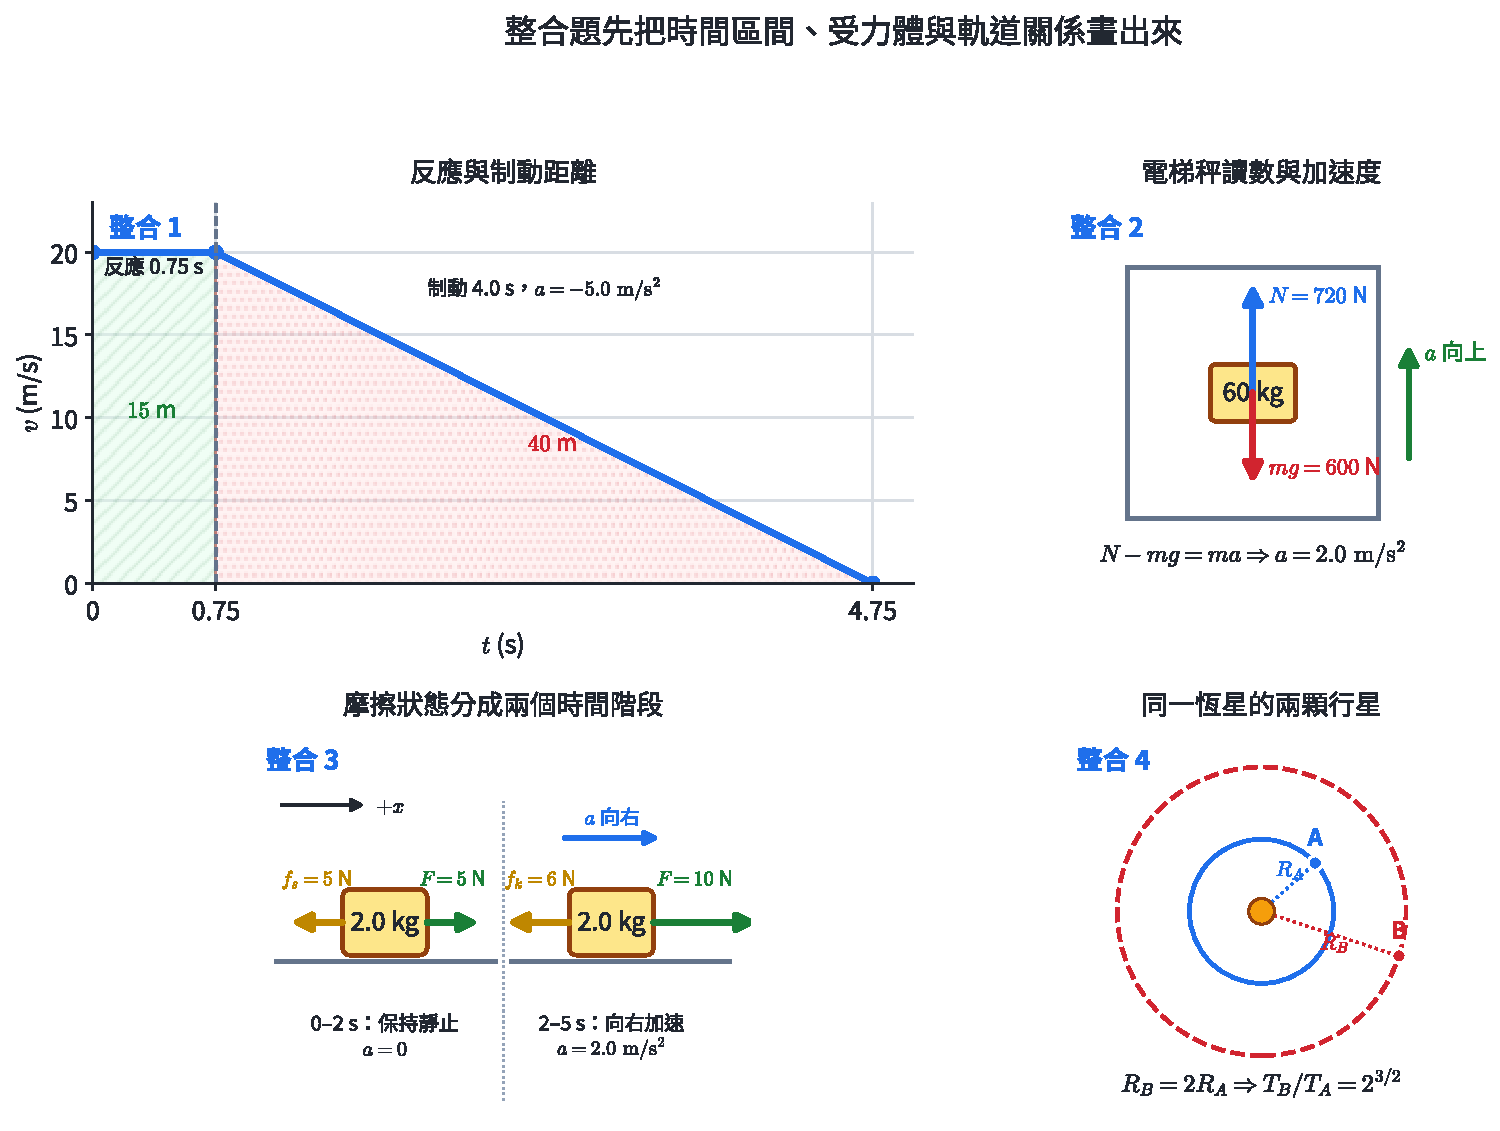
\includegraphics[width=0.98\linewidth,height=\textheight,keepaspectratio,alt={解題圖｜A 標出反應與制動的時間分界及兩塊位移面積；B 依 720:600 畫出電梯內的人所受兩力；C 分別畫出靜止與滑動兩階段；D 用半徑線標示同一恆星兩軌道的 R\_B=2R\_A。}]{assets/必物-3-章末解題圖.pdf}
\caption{解題圖｜A 標出反應與制動的時間分界及兩塊位移面積；B 依 \(720:600\) 畫出電梯內的人所受兩力；C 分別畫出靜止與滑動兩階段；D 用半徑線標示同一恆星兩軌道的 \(R_B=2R_A\)。}
\end{figure}

\subsection{第 1 題}\label{ux7b2c-1-ux984c}

首尾座標為 \(-20\ \mathrm m\) 與 \(-4\ \mathrm m\)：

\[
\Delta x=-4-(-20)=+16\ \mathrm m.
\]

兩段路徑長分別是 \(|12-(-20)|=32\ \mathrm m\) 與 \(|-4-12|=16\ \mathrm m\)，所以

\[
s=32+16=48\ \mathrm m.
\]

\[
\bar v=\frac{16}{12.0}=+1.33\ \mathrm{m/s},
\qquad
\bar u=\frac{48}{12.0}=4.00\ \mathrm{m/s}.
\]

平均速度的正號對應向 \(+x\)；平均速率使用全路徑長。

\subsection{第 2 題}\label{ux7b2c-2-ux984c}

\[
a=\frac{v_f-v_i}{\Delta t}
=\frac{2.0-(-4.0)}{2.0}
=+3.0\ \mathrm{m/s^2}.
\]

由 \(v=-4.0+3.0t\)，令 \(v=0\) 得 \(t=4/3\ \mathrm s\)。在此之前 \(v<0\)、\(a>0\)，速率由 \(4.0\ \mathrm{m/s}\) 降至零；之後 \(v>0\)、\(a>0\)，速率由零增至 \(2.0\ \mathrm{m/s}\)。速度穿越零表示運動方向反轉。

\subsection{第 3 題}\label{ux7b2c-3-ux984c}

圖 3A 的三段斜率為

\[
v_1=\frac{4-(-2)}{2}=+3\ \mathrm{m/s},
\]

\[
v_2=\frac{4-4}{5-2}=0,
\qquad
v_3=\frac{-2-4}{8-5}=-2\ \mathrm{m/s}.
\]

首尾位置都是 \(-2\ \mathrm m\)，所以 \(\Delta x=0\)，\(\bar v=0/8=0\)。路徑長為 \(6+0+6=12\ \mathrm m\)。

\subsection{第 4 題}\label{ux7b2c-4-ux984c}

圖 3B 的斜率為

\[
a=\frac{6-2}{4}=1.0\ \mathrm{m/s^2}.
\]

圖下面積為

\[
\Delta x=(2)(4)+\frac{1}{2}(4)(4)=16\ \mathrm m.
\]

\[
\bar v=\frac{\Delta x}{\Delta t}=\frac{16}{4}=4.0\ \mathrm{m/s}.
\]

線性變化的端點平均 \((2+6)/2=4.0\ \mathrm{m/s}\) 也得到同一結果。

\subsection{第 5 題}\label{ux7b2c-5-ux984c}

取向下為正。由靜止釋放，

\[
20=\frac{1}{2}(10)t^2
\Rightarrow t=2.0\ \mathrm s.
\]

當時

\[
v=gt=(10)(2.0)=20\ \mathrm{m/s},
\]

方向向下。以平均速度 \(10\ \mathrm{m/s}\) 乘 \(2.0\ \mathrm s\)，位移為 \(20\ \mathrm m\)，與已知高度相符。

\subsection{第 6 題}\label{ux7b2c-6-ux984c}

從地面參考系看，球原本靜止，又幾乎沒有水平合力，因此初期保持接近靜止。台車向右加速後會移到球的右側。

從車上看，參考系本身向右加速，球相對於車向左移動。兩個描述對應同一件事：球維持原運動狀態，車改變了速度。

\subsection{第 7 題}\label{ux7b2c-7-ux984c}

\[
m=\frac{F}{a}=\frac{4.0}{2.0}=2.0\ \mathrm{kg}.
\]

合力改為 \(6.0\ \mathrm N\) 時，

\[
a=\frac{6.0}{2.0}=3.0\ \mathrm{m/s^2}.
\]

合力與加速度的增加比例均為 \(1.5\)。

\subsection{第 8 題}\label{ux7b2c-8-ux984c}

第三定律給出 B 對 A 的力為 \(180\ \mathrm N\) 向左。取向右為正：

\[
a_A=\frac{-180}{50}=-3.6\ \mathrm{m/s^2},
\]

\[
a_B=\frac{+180}{75}=+2.4\ \mathrm{m/s^2}.
\]

力對大小相等、方向相反；加速度的不同來自兩人質量不同。

\subsection{第 9 題}\label{ux7b2c-9-ux984c}

受力圖包含向下重力 \(mg\)、向上正向力 \(N\)、向右推力 \(20\ \mathrm N\) 與向左摩擦力 \(5.0\ \mathrm N\)。鉛直無加速度：

\[
N-mg=0\Rightarrow N=(3.0)(10)=30\ \mathrm N.
\]

水平方向：

\[
20-5.0=(3.0)a
\Rightarrow a=5.0\ \mathrm{m/s^2}\text{ 向右}.
\]

\subsection{第 10 題}\label{ux7b2c-10-ux984c}

箱子靜止，鉛直合力為零。受力為 \(N\) 向上，\(mg=50\ \mathrm N\) 與手掌作用力 \(15\ \mathrm N\) 向下：

\[
N-mg-15=0,
\]

\[
N=50+15=65\ \mathrm N.
\]

額外向下力增加地面需提供的支撐。

\subsection{第 11 題}\label{ux7b2c-11-ux984c}

\[
\Delta L=4.0\ \mathrm{cm}=0.040\ \mathrm m,
\]

\[
F_s=k\Delta L=(150)(0.040)=6.0\ \mathrm N.
\]

彈簧被拉長時，它對右端物體的力指向左，使右端趨向自然長度位置。

\subsection{第 12 題}\label{ux7b2c-12-ux984c}

外力 \(7.0\ \mathrm N<f_{s,\max}\) 時，靜摩擦力自動取 \(7.0\ \mathrm N\) 且方向相反：

\[
F_{\mathrm{net}}=7.0-7.0=0,
\qquad a=0.
\]

外力 \(10\ \mathrm N>f_{s,\max}\) 時，物體滑動，摩擦力大小為 \(6.0\ \mathrm N\)：

\[
F_{\mathrm{net}}=10-6.0=4.0\ \mathrm N,
\qquad
a=\frac{4.0}{2.0}=2.0\ \mathrm{m/s^2}.
\]

加速度方向與 \(10\ \mathrm N\) 外力同向。

\subsection{第 13 題}\label{ux7b2c-13-ux984c}

使用圖 10A 的切向與徑向關係：

\begin{itemize}
\tightlist
\item
  最右端：逆時針切向為向上，所以速度向上；圓心在左，所以加速度與合力向左。
\item
  最上端：逆時針切向為向左，所以速度向左；圓心在下，所以加速度與合力向下。
\end{itemize}

速度與加速度在這兩個位置都互相垂直。

\subsection{第 14 題}\label{ux7b2c-14-ux984c}

根據克卜勒第二定律，相等時間掃過相等面積，所以 C--D 也掃過面積 \(S\)。

近日點的太陽---行星距離較短。在掃過面積與時間都相同的條件下，A--B 的軌道弧長較長，平均速率也較大；C--D 弧長較短，平均速率較小。

\subsection{第 15 題}\label{ux7b2c-15-ux984c}

繞同一恒星時，

\[
\frac{a_A^3}{T_A^2}=\frac{a_B^3}{T_B^2},
\]

\[
\left(\frac{T_B}{T_A}\right)^2
=\left(\frac{a_B}{a_A}\right)^3
=4^3=64,
\]

\[
\frac{T_B}{T_A}=8.
\]

\subsection{第 16 題}\label{ux7b2c-16-ux984c}

逐一計算：

\[
\left(\frac{a^3}{T^2}\right)_P=\frac{1^3}{1^2}=1,
\qquad
\left(\frac{a^3}{T^2}\right)_Q=\frac{4^3}{8^2}=1,
\]

\[
\left(\frac{a^3}{T^2}\right)_R=\frac{9^3}{27^2}=1.
\]

三者比值相同，支持繞同一中心天體時 \(a^3/T^2\) 為常數。從這組資料找出共同關係是歸納。

\subsection{整合題 1}\label{ux6574ux5408ux984c-1}

解題圖 A 將反應期間畫成高 \(20\ \mathrm{m/s}\)、寬 \(0.75\ \mathrm s\) 的長方形：

\[
d_r=(20)(0.75)=15\ \mathrm m.
\]

制動時間由 \(0=20+(-5.0)t_b\) 得 \(t_b=4.0\ \mathrm s\)。制動區是底 \(4.0\ \mathrm s\)、高 \(20\ \mathrm{m/s}\) 的三角形：

\[
d_b=\frac{1}{2}(4.0)(20)=40\ \mathrm m.
\]

\[
d_{\mathrm{total}}=15+40=55\ \mathrm m.
\]

\(v\)--\(t\) 圖的兩塊面積分別對應反應與制動位移。

\subsection{整合題 2}\label{ux6574ux5408ux984c-2}

使用解題圖 B，以人為受力體，向上正向力 \(N=720\ \mathrm N\)，向下重力 \(mg=(60)(10)=600\ \mathrm N\)。取向上為正：

\[
N-mg=ma,
\]

\[
720-600=60a
\Rightarrow a=+2.0\ \mathrm{m/s^2}.
\]

一秒後的速度為

\[
v=v_0+at=-3.0+(2.0)(1.0)=-1.0\ \mathrm{m/s}.
\]

末速度仍為負，電梯仍向下移動；速率由 \(3.0\) 降為 \(1.0\ \mathrm{m/s}\)。加速度向上且速度向下，因此速率減小。

\subsection{整合題 3}\label{ux6574ux5408ux984c-3}

第一階段，\(5.0\ \mathrm N<f_{s,\max}\)，靜摩擦力為 \(5.0\ \mathrm N\) 向左：

\[
F_{\mathrm{net},1}=5.0-5.0=0,
\qquad a_1=0.
\]

物體在這 \(2.0\ \mathrm s\) 保持靜止，\(v_1=0\)、\(\Delta x_1=0\)。

第二階段，\(10\ \mathrm N>f_{s,\max}\)，物體滑動，\(f_k=6.0\ \mathrm N\) 向左：

\[
F_{\mathrm{net},2}=10-6.0=4.0\ \mathrm N,
\qquad
a_2=\frac{4.0}{2.0}=2.0\ \mathrm{m/s^2}.
\]

這階段從靜止開始且維持 \(3.0\ \mathrm s\)：

\[
v_f=0+(2.0)(3.0)=6.0\ \mathrm{m/s},
\]

\[
\Delta x_2=\frac{1}{2}(2.0)(3.0)^2=9.0\ \mathrm m.
\]

全程位移為 \(9.0\ \mathrm m\) 向右，末速度為 \(6.0\ \mathrm{m/s}\) 向右。

\subsection{整合題 4}\label{ux6574ux5408ux984c-4}

使用解題圖 D。兩行星繞同一恒星，所以

\[
\left(\frac{T_B}{T_A}\right)^2
=\left(\frac{R_B}{R_A}\right)^3
=2^3=8.
\]

\[
T_B=T_A\sqrt8
=(3.00)(2\sqrt2)
\approx8.49\ \text{年}.
\]

觀測值 \(8.5\) 年與模型預測 \(8.49\) 年相符。在給定量測精度下，這份結果支持繞同一中心天體時 \(T^2\propto R^3\) 的關係。


\end{document}
